\section{Design and Implementation}
\label{sec:design}


\subsection{Datasets}
\label{subsec:project_settings_datasets}
The Boston Housing dataset was used, which aims to predict the median house price given a number of demographic features. There were 506 examples, each containing 13 input variables (12 continuous, 1 binary) and 1 continuous output variable in the range $0$ to $50$. All input variables were linearly rescaled to $[0, 1]$, independently of one another. The output variable was linearly rescaled to $[-1, 1]$. The data were converted to batches of PyTorch tensors with a batch size of $32$ ($506$ for Section~\ref{subsec:stage_4} only). 


\subsection{Model Architecture Representation}
MLP architecture was varied to introduce different model complexities. MLPs differed in architectures in terms of numbers of hidden nodes and hidden layers. A MLP could have $2$, $6$ or $12$ hidden nodes in each hidden layer. A MLP could have $1$, $3$ or $6$ hidden layers. If a MLP had more than 1 hidden layer, the number of hidden nodes in each hidden layer was fixed to $2$. The idea was to make sure the MLPs of different model architectures to be compared have the same possible total numbers of hidden nodes, which were $2$, $6$ or $12$ in the experiment. 

The model architecture was represented by a Python list. The table below contained all model architectures used in this project: 

\begin{table}[H]
    \centering
    \begin{tabular}{|c|c|}
        \hline
        Model architecture & Description \\
        \hline
        \small\texttt{[2]} & 1 hidden layer of 2 hidden nodes \\
        \hline
        \small\texttt{[2, 2, 2]} & 3 hidden layers of 2 hidden nodes \\
        \hline
        \small\texttt{[2, 2, 2, 2, 2, 2]} & 6 hidden layers of 2 hidden nodes \\
        \hline
        \small\texttt{[6]} & 1 hidden layer of 6 hidden nodes \\
        \hline
        \small\texttt{[12]} & 1 hidden layer of 12 hidden nodes \\
        \hline
    \end{tabular}
    \caption{Overview of the neural network model architectures used in the experiments}
    \label{table:background_model_architecture}
\end{table}


\subsection{Experiment Data and Graph Generation}
To ensure flexibility, all experiments were conducted in two steps. The first step generated experimental data and outputted a \texttt{csv} file while the second step produced the corresponding graphs from this output. This design enabled graph generation without re-running experiments. Experiment graphs were generated using the \texttt{plot} function from the Python visualisation library \texttt{Matplotlib}. 


\subsection{Develop Baseline Models}
\label{subsec:stage_1}
\label{subsec:stage_2}
\paragraph{Motivation}
A single MLP is often unreliable because it may fail to fully capture the data patterns regardless of training time. In real life, critical decisions are usually made by a committee rather than one person. By applying this to machine learning, multiple models can "average out" individual errors. With the right aggregation method, the final prediction of an ensemble model becomes more reliable and less sensitive to noise. In this stage, a MLP and an arithmetic-mean-ensemble is implemented. 

This leads to the current primary research question: how much more accurate is a ``committee of directors'' compared to the decision of a single ``chairman''? 


\paragraph{Model Construction}
Object-Oriented Programming was adopted to improve maintainability and reusability. In the first part, a custom MLP class (\texttt{MLP}) was implemented by extending \texttt{torch.nn.Module}, the base class for PyTorch neural networks. Each layer was fully connected, implemented using paired lists of \texttt{torch.nn.Linear} layers and activation functions (e.g. \texttt{torch.nn.ReLU}), with equal length. Predictions were generated by sequentially applying \texttt{activation\_function(linear\_layer(...))} across all layers. The class also provided helper methods to construct MLPs from alternative specifications, e.g. layer sizes or NEAT-Python genome instances. MLPs of different configurations are trained with different randomly-shuffled datasets. 

In the second part, base learners within the ensemble (\texttt{TraditionalBaseLearner}) were derived from \texttt{MLP}, utilising the same loss function while incorporating new attributes for distributed execution, e.g. \texttt{rank} and \texttt{device\_rank}. To leverage the dual-GPU architecture of CSF3, all base learners were partitioned across two devices. Each learner was uniquely identified by a \texttt{rank:device\_index} tuple, where \texttt{rank} specified the global GPU ID and \texttt{device\_index} denoted the local learner position on that hardware. To maximise computational throughput, \texttt{torch.cuda.stream} was implemented, enabling concurrent execution of multiple base learners on a single GPU rather than sequential processing. Base learners were initialised randomly but trained with the same dataset. 

The ensemble model (\texttt{TraditionalEnsembleNet}) functioned as a central coordinator for multiple 
\\
\texttt{TraditionalBaseLearner} instances. The system leveraged PyTorch modules \texttt{DistributedDataParallel} (DDP) and \texttt{Multiprocessing} for process management and inter-device communication in such distributed environment. The execution workflow utilised \texttt{torch.multiprocessing.spawn} to initialise individual learner processes while \texttt{torch.distributed.init\_process\_group} enabled communication across GPUs. This infrastructure enabled \texttt{torch.distributed.all\_gather} to synchronise and collect predictions from every base learner despite their host GPU. Collected predictions were managed via a 
\\
\texttt{torch.multiprocessing.Manager().Queue()}, providing a thread-safe shared memory space for data aggregation. Finally, the ensemble computed the arithmetic mean of all base learner predictions using an aggregator class \texttt{ArithmeticMeanVoter}. Below contains the steps of ensemble model prediction: 
\begin{enumerate}
    \item \textbf{Getting input tensor} \\
    An input tensor is passed to the ensemble model. 

    \item \textbf{Creating base learners} \\
    If processes of base learners are not created, they are created in all available GPUs using 
    \\
    \texttt{torch.multiprocessing.spawn} and \texttt{torch.distributed.init\_process\_group} etc. Otherwise, the existing base learners are used. 

    \item \textbf{Simultaneous individual predictions} \\
    The input tensor is broadcasted to every base learner and each learner calculates their predictions simultaneously. 

    \item \textbf{Aggregating individual predictions} \\
    All base learners are blocked before their next prediction until all learners have completed their predictions, which is achieved using \texttt{torch.distributed.all\_gather} and \texttt{torch.cuda.synchronize()}. All predictions are then passed to CPU for aggregation. In training mode, all base learners are then updated using backpropagation. 

    \item \textbf{Output predictions} \\
    The aggregated prediction is returned. 

    \item \textbf{Termination} \\
    Steps 1-5 are repeated until all input data have been read. 
\end{enumerate}


\paragraph{Experimental Design for MLP}
In this experiment, \texttt{torch.optim.Adam} was chosen for its rapid convergence. Alternative optimisers and hyperparameter settings (e.g. learning rate) could be explored with additional time. The motivation for the use of ReLU is discussed in Section~\ref{subsubsec:dynamic_nn_on_gpu}. To exploit parallelism, all models were trained on CSF3 \textit{A100 GPUs}. For efficiency, each epoch computed training loss, then temporarily switched to evaluation mode to measure testing loss before resuming training. Table~\ref{table:experiment_1_varied_hyperparameters} contains all varied hyperparameters. Table~\ref{table:experiment_1_fixed_hyperparameters} contains all fixed hyperparameters. Table~\ref{table:experiment_1_metric} contains all evaluation metrics collected in this experiment. 

\begin{table}[H]
    \centering
    \begin{tabular}{|c|c|p{5cm}|c|}
        \hline
        Hyperparameter & Type & Choices / Ranges & Description \\
        \hline
        \small\texttt{epoch\_nums} & Integer & $[10, 1000]\text{, step}=10$ & Number of training epochs \\
        \hline
        \small\texttt{hidden\_sizes} & Python list & \{\texttt{[2]}, \texttt{[2, 2, 2]}, \texttt{[2, 2, 2, 2, 2, 2]}, \texttt{[6]}, \texttt{[12]}\} & Model architecture \\
        \hline
    \end{tabular}
    \caption{Varied hyperparameters and their configurations}
    \label{table:experiment_1_varied_hyperparameters}
\end{table}

\begin{table}[H]
    \centering
    \begin{tabular}{|c|c|c|p{5cm}|}
        \hline
        Hyperparameter & Type & Choices / Ranges & Description \\
        \hline
        \small\texttt{input\_size} & Integer & $13$ & Number of input features of the MLP \\
        \hline
        \small\texttt{output\_size} & Integer & $1$ & Number of labels of the MLP \\
        \hline
        \small\texttt{optimizer} & Categorical & \texttt{torch.optim.Adam} & Optimisation algorithm used for training \\
        \hline
        \small\texttt{learning\_rate} & Float & $0.0001$ & Learning rate of the optimisation algorithm \\
        \hline
        \small\texttt{dropout\_rate} & Float & $0$ & Dropout rate applied to the data tensor after the input layer \\
        \hline
        \small\texttt{activation} & Categorical & ReLU & Activation function used in each dense layer of the MLP \\
        \hline
        \small\texttt{batch\_size} & Integer & $32$ & Number of training samples passed to the model in one go \\
        \hline
    \end{tabular}
    \caption{Fixed hyperparameters and their configurations}
    \label{table:experiment_1_fixed_hyperparameters}
\end{table}

\begin{table}[H]
    \centering
    \begin{tabular}{|c|c|c|}
        \hline
        Metric & Type & Description \\
        \hline
        \small\texttt{loss\_test} & Float & MSE of MLP during testing \\
        \hline
        \small\texttt{loss\_train} & Float & MSE of MLP during training \\
        \hline
    \end{tabular}
    \caption{Evaluation metrics}
    \label{table:experiment_1_metric}
\end{table}


\paragraph{Experimental Design for arithmetic-mean-ensemble}
Experiments had been conducted to compare the performance of the two models. In the arithmetic-mean-ensemble, all base learners were trained independently. It was essentially an arithmetic-mean-aggregator of all base learners, i.e. $\hat{y}_{ensemble} = \frac{1}{m} \sum_{i=1}^{m} \hat{y}_i$. The control MLP was to serve as a reference point of the ensemble performance and had the same hyperparameter configurations (e.g. model complexity) as each ensemble learner for fair comparisons. Each ensemble was evaluated exclusively against a control MLP that shared an identical architecture and training duration, ensuring that any observed performance gains were due to the use of ensembling rather than individual base learner superiority. Furthermore, to maintain experimental focus, standard variance-reduction techniques such as \textit{bagging} were omitted from the training phase. Table~\ref{table:experiment_2_varied_hyperparameters} contains all varied hyperparameters. Table~\ref{table:experiment_2_fixed_hyperparameters} contains all fixed hyperparameters. Table~\ref{table:experiment_2_metric} contains all evaluation metrics collected in this experiment. 

\begin{table}[H]
    \centering
    \begin{tabular}{|c|c|p{5cm}|c|}
        \hline
        Hyperparameter & Type & Choices / Ranges & Description \\
        \hline
        \small\texttt{ensemble\_sizes} & Integer & $[2, 16]\text{, step}=1$ & $m$ \\
        \hline
        \small\texttt{epoch\_nums} & Integer & \{$200$, $400$\} & Number of training epochs \\
        \hline
        \small\texttt{hidden\_sizes} & Python list & \{\texttt{[2]}, \texttt{[2, 2, 2]}, \texttt{[2, 2, 2, 2, 2, 2]}, \texttt{[6]}, \texttt{[12]}\} & Model architecture \\
        \hline
    \end{tabular}
    \caption{Varied hyperparameters and their configurations}
    \label{table:experiment_2_varied_hyperparameters}
\end{table}

\begin{table}[H]
    \centering
    \begin{tabular}{|c|c|c|p{5cm}|}
        \hline
        Hyperparameter & Type & Choices / Ranges & Description \\
        \hline
        \small\texttt{input\_size} & Integer & $13$ & Number of input features of the MLP \\
        \hline
        \small\texttt{output\_size} & Integer & $1$ & Number of labels of the MLP \\
        \hline
        \small\texttt{optimizer} & Categorical & \texttt{torch.optim.Adam} & Optimisation algorithm used for training \\
        \hline
        \small\texttt{learning\_rate} & Float & $0.001$ & Learning rate of the optimisation algorithm \\
        \hline
        \small\texttt{dropout\_rate} & Float & $0.5$ & Dropout rate applied to the data tensor after the input layer \\
        \hline
        \small\texttt{activation} & Categorical & ReLU & Activation function used in each dense layer of the MLP \\
        \hline
        \small\texttt{voter} & Categorical & \texttt{arithmetic\_mean} & Type of aggregator used to combine base learners' predictions \\
        \hline
        \small\texttt{batch\_size} & Integer & $32$ & Number of training samples passed to the model in one go \\
        \hline
    \end{tabular}
    \caption{Fixed hyperparameters and their configurations}
    \label{table:experiment_2_fixed_hyperparameters}
\end{table}

\begin{table}[H]
    \centering
    \begin{tabular}{|c|c|c|}
        \hline
        Metric & Type & Description \\
        \hline
        \small\texttt{loss\_test} & Float & MSE of ensemble model during testing \\
        \hline
        \small\texttt{diversity\_coefficient\_test} & Float & $\rho$ during testing \\
        \hline
        \small\texttt{loss\_test\_base\_learner} & Float & Average MSE of base learner during testing \\
        \hline
    \end{tabular}
    \caption{Evaluation metrics}
    \label{table:experiment_2_metric}
\end{table}


\subsection{Implement NCL Ensemble}
\label{subsec:stage_3}
\paragraph{Motivation}
In the previous design (Section~\ref{subsec:stage_2}), model configurations relied on passive diversity by initialising base learners differently using randomness. While diversity is essential for ensemble performance, traditional techniques like bagging only encourage this diversity indirectly. This stage investigates whether we can take a more proactive approach by actively penalising base learners for being too similar to one another. However, excessive focus on diversity can be counterproductive, potentially degrading ensemble performance. Thus, an optimal balance between individual learner accuracy and collective diversity must be achieved. Negative Correlation Learning is explored as a mechanism for more granular control over this trade-off. 

This brings us to the next stage of our analogy: how does the quality of a decision-making change when company directors are explicitly forced to have different opinions? 


\paragraph{Model Construction}
The architectural framework remained consistent with Section~\ref{subsec:stage_2}, with the primary modification residing in the base learners' loss function. To explicitly encourage model divergence, the standard squared loss was augmented with a correlation penalty term that discouraged similarity between individual learners. $\lambda$ was introduced to manage the trade-off between individual accuracy and ensemble diversity. 


\paragraph{Experimental Design}
Experiments had been conducted to mainly compare the performance of a NCL ensemble model and that of an arithmetic-mean-ensemble (the performance of a MLP was also included for reference). The experiment settings were identical to those in Section~\ref{subsec:stage_2} except a NCL ensemble model was added to the experiment too. In the NCL ensemble model, all base learners were trained using NCL. To ensure comparison fairness, each NCL ensemble model was evaluated exclusively against a control MLP that shared an identical architecture and training duration (epoch count). This ensured that any observed performance gains were due to the diversity rather than individual architectural advantages. Table~\ref{table:experiment_3_varied_hyperparameters} contains all varied hyperparameters. Table~\ref{table:experiment_3_fixed_hyperparameters} contains all fixed hyperparameters. Table~\ref{table:experiment_3_metric} contains all evaluation metrics collected in this experiment. 

\begin{table}[H]
    \centering
    \begin{tabular}{|c|c|p{4cm}|c|}
        \hline
        Hyperparameter & Type & Choices / Ranges & Description \\
        \hline
        \small\texttt{correlation\_penalty\_coefficients} & Float & $[0, 1.5]\text{, step}=0.1$ & $\lambda$ \\
        \hline
        \small\texttt{ensemble\_sizes} & Integer & $[2, 16]\text{, step}=1$ & $m$ \\
        \hline
        \small\texttt{hidden\_sizes} & Python list & \{\texttt{[2]}, \texttt{[2, 2, 2]}, \texttt{[2, 2, 2, 2, 2, 2]}, \texttt{[6]}, \texttt{[12]}\} & Model architecture \\
        \hline
    \end{tabular}
    \caption{Varied hyperparameters and their configurations}
    \label{table:experiment_3_varied_hyperparameters}
\end{table}

\begin{table}[H]
    \centering
    \begin{tabular}{|c|c|c|p{5cm}|}
        \hline
        Hyperparameter & Type & Choices / Ranges & Description \\
        \hline
        \small\texttt{input\_size} & Integer & $13$ & Number of input features of the MLP \\
        \hline
        \small\texttt{output\_size} & Integer & $1$ & Number of labels of the MLP \\
        \hline
        \small\texttt{optimizer} & Categorical & \texttt{torch.optim.Adam} & Optimisation algorithm used for training \\
        \hline
        \small\texttt{learning\_rate} & Float & $0.001$ & Learning rate of the optimisation algorithm \\
        \hline
        \small\texttt{dropout\_rate} & Float & $0.5$ & Dropout rate applied to the data tensor after the input layer \\
        \hline
        \small\texttt{activation} & Categorical & ReLU & Activation function used in each dense layer of the MLP \\
        \hline
        \small\texttt{epoch\_nums} & Integer & $400$ & Number of training epochs \\
        \hline
        \small\texttt{voter} & Categorical & \texttt{arithmetic\_mean} & Type of aggregator used to combine base learners' predictions \\
        \hline
        \small\texttt{batch\_size} & Integer & $32$ & Number of training samples passed to the model in one go \\
        \hline
    \end{tabular}
    \caption{Fixed hyperparameters and their configurations}
    \label{table:experiment_3_fixed_hyperparameters}
\end{table}

\begin{table}[H]
    \centering
    \begin{tabular}{|c|c|c|}
        \hline
        Metric & Type & Description \\
        \hline
        \small\texttt{loss\_test} & Float & MSE of ensemble model during testing \\
        \hline
        \small\texttt{diversity\_coefficient\_test} & Float & $\rho$ during testing \\
        \hline
    \end{tabular}
    \caption{Evaluation metrics}
    \label{table:experiment_3_metric}
\end{table}


\paragraph{Reference Experiment}
The experiment on NCL ensemble model was based on the NCL experiments on the Boston Housing dataset conducted in Brown et al.\ \cite{brown2005managing}. It aimed at reproducing similar experiment results to study the effect of correlation penalty coefficient (represented as $\gamma$ in Brown et al.\ \cite{brown2005managing}) on NCL ensemble loss. To extend the experiment, three extensions had been added to the NCL experiment in this work. 

In order to better compare the performance of NCL ensemble model and the original performance, MSE of a control MLP had been added. Although varying $\lambda$ did not affect the performance of the control MLP and the arithmetic-mean-ensemble (from Section~\ref{subsec:stage_2}), having a control MLP and a control arithmetic-mean-ensemble enable the visualisation of the performance improvement of NCL ensemble models at different values of $\lambda$. Furthermore, as mentioned in Brown et al.\ \cite{brown2005managing}, the upper bound of $\lambda$ could be larger than $1$ if the ensemble size was small enough (e.g. $\lambda = 2$). Thus, the NCL experiment extended the range of $\lambda$ from $[0, 1]$ to $[0, 1.5]$, allowing us to study the NCL ensemble performance for $\lambda$ slightly beyond $1$. Lastly, there were 2 ways of varying the model complexity. In Brown et al.\ \cite{brown2005managing}, model complexity was increased by adding more hidden nodes to the neural network but each neural network always had 1 hidden layer. In this project, model could get more complex by either increasing the number of hidden nodes (then all models always had 1 hidden layer) or the number of hidden layers (then always 2 hidden nodes for each hidden layer). Similar to the reference experiments, early stopping is configured. In the current experiments, it never happened. 

There are 2 categories for the experiment figures. One category provides comparisons of the impacts of $\lambda$ on MSE and diversity coefficient across particular ensemble models with a fixed model architecture. The other category provides comparisons of the impacts of $\lambda$ on MSE and diversity coefficient across particular ensemble models with a fixed ensemble size. Furthermore, when $\lambda$ exceeded an upper bound, ensemble MSE and diversity coefficient increased exponentially. If $\lambda$ in a graph had range $[0, 1.5]$, it would be difficult to compare the MSE and diversity coefficient for smaller values of $\lambda$. Thus, $\lambda$ in graphs either have range $[0, 1]$ or $[0.8, 1.5]$ so that MSE and diversity coefficient comparisons can be viewed more clearly. 


\subsection{Integrate NEAT with NCL}
\label{subsec:stage_4}
\paragraph{Motivation}
In the previous design (Section~\ref{subsec:stage_3}), diversity was explicitly enforced through NCL, under the assumption that all base learners shared a uniform architecture (MLPs with identical topologies and hidden nodes). In that context, diversity was derived solely from variations in weights. This stage moves beyond weight-based variation to explore the impact of architectural diversity. We investigate how structural differences between base learners affect overall ensemble performance and aim to identify the optimal architecture for this specific problem. Furthermore, the objective in Section~\ref{subsec:stage_3} also tests the hypothesis that different ensembles have different optimal values of correlation penalty coefficient ($\lambda^*$). This stage addresses such challenge and determines $\lambda$ dynamically based on diversity rather than exhaustive manual tuning. 

This brings us to the next stage of our analogy: how does the quality of a decision making change if the company committee includes members with entirely different backgrounds and ``species'' of thought (e.g. both animals and human) rather than just different opinions? 


\subsubsection{NEAT-NCL algorithm}
The traditional NEAT algorithm (mentioned in Section~\ref{subsec:background_neat}) was modified. Between \textit{reproduction} and \textit{replacement}, a step of \textit{backpropagation with NCL} was added. Then, the fitness of each base learner was updated before \textit{replacement}. 

Below contains the steps of the algorithm: 
\begin{enumerate}
    \item \textbf{Initialisation} \\
    An initial population of $m$ neural network base learners is generated. Each base learner is encoded using graph encoding represented by a collection of nodes and edges. The number of hidden neurons, connections and connection weights in the base learners are initialised randomly. Based on the configurations, the initial number of connections and their weights can be partially controlled. 

    \item \textbf{Evaluation} \\
    The raw fitness of each base learner in the population is computed using the equation below: 

    \begin{equation}
        \label{equation:neat_ncl_raw_fitness}
        fitness = (\hat{y}_i - y)^2 - (\hat{y}_i - \bar{y})^2 + \sum_{ij} \frac{weight_{ij}^2}{1 + weight_{ij}^2}
    \end{equation}

    where $\hat{y}_i$ is the prediction made by the $i$th base learner, $\bar{y}$ is the mean prediction of all base learners, $y$ is the true value. The third term is a weight decay, which is used to estimate the architectural complexity of the base learner and improve the generalisation of base learners. $weight_{ij}$ denotes the connection weight from Neuron $i$ to Neuron $j$. 

    To maintain population diversity and prevent premature convergence, fitness sharing is implemented. In traditional fitness sharing, the niche radius is pre-computed. In most real applications, there is no prior knowledge about fitness landscape available and it is difficult to set the niche radius appropriately. In this experiment, the niche radius $\sigma$ is computed dynamically using the equation below: 
    
    \begin{equation}
        \label{equation:neat_ncl_niche_radius}
        \sigma = \frac{1}{2 m^2} \sum_{i = 1}^{m} \sum_{j = 1}^{m} distance_{ij}
    \end{equation}

    where $m$ is the ensemble size, i.e. population size. $distance_{ij}$ is the genetic distance between the $i$th and $j$ base learners. To compute the genetic distance between 2 base learners, Equation~\ref{equation:neat_ncl_genetic_distance} is used. 
    
    Below contains the pseudo-code used to update the raw fitness of 1 base learner by taking into account sharing factor during fitness sharing: 

    \begin{lstlisting}[language=Python, caption={Modified fitness sharing}]
    # The sharing factor of current_base_learner
    sharing_factor = 0
    # Calculate the dynamic niche radius based on the current ensemble size m
    sigma = get_dynamic_niche_radius(m)
    # A scaling factor pre-computed by developers
    alpha = 1

    for other_base_learner in population where other_base_learner is not current_base_learner:
        d = get_genetic_distance(current_base_learner, other_base_learner)

        if d < sigma:
            # current_base_learner is genetically too close to other_base_learner
            sharing_factor += 1 - (d / sigma) ** alpha
        
    # sharing_factor is ready

    # Update the raw fitness of the current base learner for fitness sharing
    current_base_learner.fitness = current_base_learner.fitness / sharing_factor
    \end{lstlisting}
    The fitness of every base learner is updated using the above algorithm. The updated fitness is called \textit{adjusted fitness}. 

    \item \textbf{Selection} \\
    Based on the adjusted fitness, stronger parent genomes are selected. Crossover among dissimilar individuals often produces low-performance offsprings. Thus, the selection process is modified. Specifically, during selection, parent genomes are ranked in descending order of their adjusted fitness values. $P_1$ and $P_2$, which have the 2 highest fitness values, will be mated. Then, $P_3$ and $P_4$ are mated and so on. When there are not enough offspring genomes produced after reaching the bottom of the population, the pointers go back and $P_1$ and $P_2$ are mated again and so on. 

    \item \textbf{Reproduction} \\
    Crossover and mutation on selected paired parent genomes are applied to generate stronger intermediate offsprings. 

    \item \textbf{Backpropagation with NCL} \\
    Backpropagation with NCL is applied to intermediate offsprings to update their connection weights. Each offspring has the loss function specified in Equation~\ref{equation:ncl}. An appropriate value of $\lambda$ is required for such loss function, which is dynamically computed using the equation below: 
    
    \begin{equation}
        \label{equation:neat_ncl_dynamic_lambda}
        \lambda = \lambda_{max} - \frac{D}{D_{max}} \times (\lambda_{max} - \lambda_{min})
    \end{equation}

    where $\lambda_{max}$ and $\lambda_{min}$ correspond to the upper and lower bounds values of $\lambda$ set by developers ($0.1$ and $0.9$ respectively). Thus, $\lambda$ varies from $\lambda_{min}$ to $\lambda_{max}$. $D$ is the population diversity computed in the current population. $D_{max}$ is the maximum population diversity recorded in the population. 

    Equation~\ref{equation:neat_ncl_dynamic_lambda} requires $D$, which is dynamically computed (refer to Section~\ref{subsubsec:neat_ncl_population_diversity} for the calculation steps). Based on Equation~\ref{equation:neat_ncl_dynamic_lambda}, $\lambda$ is set to a very large number initially (because the initial population has little diversity, i.e. small $D$) and it is decreased gradually until it reaches its optimal value. In other words, diversity of base learners is prioritised at the beginning but accuracy receives more attention as there are more diverse genomes in the population. 

    \item \textbf{Evaluation of offsprings} \\
    The fitness of each offspring base learner is computed. The same procedure from Step 2 are applied to the new genomes created. This means the current population contains both offspring and parent genomes. 

    \item \textbf{Replacement} \\
    To maintain the size of the population to $m$, all genomes are ranked based on their values of adjusted fitness. The top $m$ genomes are selected to survive in the next generation while the remaining genomes are eliminated. Since elitism is enabled, certain ``elite'' genomes of each species are exceptionally copied directly to the next generation. 

    \item \textbf{Termination} \\
    In the current configurations, steps 2-7 are repeated until the maximum number of generations is reached. The fitness of base learners is not used to determine termination and is merely for selection. 
\end{enumerate}


\subsubsection{Population diversity Calculation}
\label{subsubsec:neat_ncl_population_diversity}
The population diversity $D$ of a population is computed using the steps below: 
\begin{enumerate}
    \item \textbf{Output distance} \\
    For each 2 genomes within a \textit{subpopulation} (a group of genomes with the same number of hidden nodes), calculate their output distance $output\_distance_{ij}$ using the equation below: 

    \begin{equation}
        \label{equation:neat_ncl_output_distance}
        output\_distance_{ij} = \frac{1}{N} \sum_{n = 1}^N \left| \hat{y}_{i,n} - \hat{y}_{j,n} \right|
    \end{equation}

    where $N$ is the number of training data. $\hat{y}_{i,n}$ and $\hat{y}_{j,n}$ are the predictions of the $i$th and $j$th networks, on the $n$th training data respectively. 

    \item \textbf{Genetic distance} \\
    For each 2 genomes within a subpopulation, calculate their genetic distance $genetic\_distance_{ij}$ (i.e. compatibility distance) using the equation below: 

    \begin{equation}
        \label{equation:neat_ncl_genetic_distance}
        genetic\_distance_{ij} = \frac{c_1 N_{excess}}{N} + \frac{c_2 N_{disjoint}}{N} + c_3 \bar{W}
    \end{equation}

    where $N_{excess}$ is the number of excess genes, $N_{disjoint}$ is the number of disjoint genes, $N$ is the number of genes in the larger genome (acting as a normalisation factor), $\bar{W}$ is the average weight difference of matching genes, $c_1$, $c_2$ and $c_3$ are coefficients controlling the importance of each term, set to $1$, $1$ and $0.5$ respectively. 

    \item \textbf{Diversity contribution} \\
    For each 2 genomes within a subpopulation, calculate their contribution to the subpopulation diversity using the equation below: 

    \begin{equation}
        \label{equation:neat_ncl_diversity_contribution}
        subpopulation\_diversity_{ij} = \frac{fitness_i + fitness_{j}}{2 \times fitness_{average}} \times genetic\_distance_{ij} \times output\_distance_{ij}
    \end{equation}

    where $f_{average}$ is the average fitness of the subpopulation. $fitness_i$ and $fitness_j$ are the fitness of the $i$th and $j$th networks respectively. 

    \item \textbf{Subpopulation diversity} \\
    For each subpopulation of the whole population, calculate the subpopulation diversity using the equation below: 

    \begin{equation}
        \label{equation:neat_ncl_subpopulation_diversity}
        subpopulation\_diversity = \frac{2}{k(k - 1)} \sum_{i = 1}^{k - 1} \sum_{j = i + 1}^k subpopulation\_diversity_{ij}
    \end{equation}

    where $k$ is the number of neural networks in the subpopulation. The sum of $k$ of all subpopulations gives $m$. Note that this formula is calculating the average subpopulation diversity. 

    \item \textbf{Population diversity} \\
    Calculate $D$ using the equation below: 

    \begin{equation}
        \label{equation:neat_ncl_population_diversity}
        population\_diversity = \sum_{i = 1}^c subpopulation\_diversity_{i}
    \end{equation}

    where $c$ is the number of subpopulations. $D$ can be treated as sum of all subpopulation diversities. 
\end{enumerate}


\paragraph{Model Construction}
The NEAT-NCL codebase was constructed upon the \textit{NEAT-Python} library, extending its core evolutionary mechanisms, e.g. selection and crossover, to support NCL. Key modifications included customised selection, fitness sharing and the integration of backpropagation with NCL post-reproduction. 

To handle the high computational overhead of iterating through genome combinations, a specialised data structure \texttt{Table} in \path{data_container.py} was implemented. This structure facilitates efficient storage and retrieval of population matrices, including: 
\begin{enumerate}
    \item \textbf{Genetic and Output Distances} \\
    Measuring structural and functional divergence. 

    \item \textbf{Subpopulation Diversity} \\
    Tracking the contribution of individual genomes to niche variety. 

    \item \textbf{Fitness Sharing} \\
    Scaling individual fitness based on the proximity of peers. 
\end{enumerate}

Algorithmic logic and statistical formulae, e.g. the sharing factor and $\sigma$ calculations, were encapsulated in \path{neat_ncl_trainer.py} and \path{maths_helper.py}. The integrity of these calculations was verified through extensive unit testing in \path{data_container_test.py} and \path{graph_helper_test.py}. 

The execution is governed by \texttt{config-housing-neat-ncl.ini}, which defines the structural and behavioural attributes of the population: 
\begin{enumerate}
    \item \textbf{Weight Initialisation} \\
    Connections use a Gaussian distribution (\lstinline|weight_init_mean = 0.0|, \lstinline|weight_init_stdev = 1.0|). 

    \item \textbf{Topology Evolution} \\
    Genomes can be initialised as \lstinline|unconnected| (no initial connections), \lstinline|full_direct| (complete input-to-output mapping) or \lstinline|partial_direct 0.5| (a $50\%$ random subset of a full-direct mapping). Complexity is added incrementally through connection mutation. 

    \item \textbf{Population Dynamics} \\
    An ensemble size of $150$ can be maintained using \lstinline|pop_size = 150| with \lstinline|elitism = 2| to preserve the best-performing genomes across generations. Species stability is ensured via \lstinline|min_species_size = 2|. 

    \item \textbf{Network Constraints} \\
    The \lstinline|feed_forward = True| setting is mandatory to support the topological evaluation algorithm described in Section~\ref{subsubsec:dynamic_nn_on_gpu}. 
\end{enumerate}

The transition from genotype to phenotype was managed by \texttt{NEATNCLBaseLearner} (\path{neat_ncl_base_learner.py}), which instantiated individual phenomes. Below contains some of its important components: 
\begin{enumerate}
    \item \textbf{Nodes and Edges} \\
    Neurons are represented by \texttt{Node} objects (\path{node.py}), identified by IDs where input neurons are strictly negative ($node\_id_{input} \in \{-1, -2, ...\}$). Weighted connections are managed via \texttt{Edge} objects (\path{edge.py}). 

    \item \textbf{Forward Pass} \\
    The \texttt{torch.nn.Module} prediction method \texttt{forward} has been re-engineered to follow a strict topological evaluation order, ensuring that signal propagation respects the dynamic nature of the evolved network. 
\end{enumerate}

The entire population was orchestrated by \texttt{NEATNCLEnsembleNet} (\path{neat_ncl_ensemble_net.py}). Its primary method, \texttt{evolve}, executed the evolutionary loop for a specified number of generations using a dictionary of parameters, e.g. $\lambda_{min}$, $\lambda_{max}$ and training partitions, to evaluate and refine genome fitness through NCL. 


\subsubsection{Dynamic neural network on GPU}
\label{subsubsec:dynamic_nn_on_gpu}
GPUs are built for massively parallel, uniform workloads. In NEAT, neural networks are evolved and their topologies change over each generation. Each NEAT individual in the population has a different architecture so uniform batch of matrix multiplications and high-throughput SIMD execution cannot be executed on GPU. However, instead of running networks on CPU, which is much slower, an algorithm has been developed to convert a dynamic neural network to a GPU-runnable representation. The goal of the algorithm is to create a different GPU-runnable neural network such that it is equivalent to the original dynamic neural network. The new regular neural network should have the correct sequential order of data flow between neurons and the correct connection weights applied to give the same final prediction as the original network. Each neural network can be treated as a DAG with nodes representing neurons and edges representing weighted connections. Essentially, the algorithm converts a DAG to a graph of nodes (fully-connected graph) such that each node is connected to every node in the next layer, i.e. a fully-connected layer. Below contains the steps of the algorithm: 
\begin{enumerate}
    \item \textbf{Topological sort} \\
    The topological sort of nodes is calculated. This creates a correct sequential order of data flow through nodes. 

    \item \textbf{Set up input neurons in the first layer} \\
    For a fully-connected layer, all input neurons must be in the first layer. New nodes are created in the first layer and connections with weight~$1$ are added to allow direct data flow from the first layer to every input neuron in the topological sort. 

    \item \textbf{Create connections} \\
    This step ensures connection weights are applied in the correct order and with the right value according to the original DAG. For every edge \texttt{(start\_node\_id, end\_node\_id)} in the DAG, the connection weight ($w$), IDs of the start and end nodes (\texttt{start\_node\_id} and \texttt{end\_node\_id}) are retrieved. The algorithm attempts to form a linking between the corresponding 2 nodes in the fully-connected graph (\texttt{start\_node} and \texttt{end\_node}). It follows 2 simple rules: 
    \begin{enumerate}
        \item \textbf{2 nodes are directly next to each other} \\
        Add a direct connection with weight~$w$ between the 2 nodes

        \item \textbf{2 nodes are not directly next to each other} \\
        For each layer between the 2 nodes, add a node at the bottom of the layer. Add connections connecting \texttt{start\_node} and \texttt{end\_node} through the newly added nodes. All connections have weights $1$ except the last connection, which has weight~$w$. 
    \end{enumerate}

    \item \textbf{Add non-functional connections} \\
    At this state, an equivalent minimum graph of nodes and edges is constructed successfully and data flows with the correct sequential orders and values. Then, a connection with weight~$0$ is added to connect every pair of nodes which does not have an existing connection yet. This ensures the final graph represents a fully-connected network and can be run on GPU using PyTorch. 

    \item \textbf{Create instances of \texttt{nn.LinearLayer} based on neuron bias and connection weight} \\
    Using the generated fully-connected graph, instances of \texttt{nn.LinearLayer} are created. An instance of \texttt{nn.LinearLayer} is represented by a matrix. They are initialised with weight~$0$ and bias~$0$ initially. All non-zero connection weights and biases are then used to update the \texttt{nn.LinearLayer} matrix at the correct positions. 
\end{enumerate}

\paragraph{Assumption}
Two assumptions have been made. There must not be recurrent connections, i.e. the network must be \textbf{feed-forward}. Furthermore, the activation function used must be \textbf{idempotent} because the algorithm expects the values of input data remain unchanged when passing every node until they reach the last connection with weight~$w$. The activation function \texttt{torch.nn.ReLU} was acceptable only when the input data are non-negative. This algorithm was not used in the experiment because it does not support backpropagation. The \textit{identity function} is also acceptable for this algorithm. 

\paragraph{Limitation}
The algorithm is \textbf{irreversible} as it can only convert a DAG to a fully-connected graph but not the other way around. Thus, after backpropagation with NCL, the weights of the fully-connected graph are updated and the DAG of the genome will no longer be updated and cannot be used for crossover for the next generation. Therefore, in this project, this algorithm is only used when the phenomes are executed in inference mode but not training mode where weights are updated via backpropagation. For training the networks and evolutionary algorithm, networks are run on CPU and this algorithm is not used, e.g. during the experiments. 
ReLU can be used in this algorithm only if every node has a non-negative value. 

\paragraph{Testing}
Unit tests in \path{algorithm_test.py} and \path{mlp_test.py} are created to test the correctness of the algorithm implementation. The model created by the algorithm is compared against that created using 
\\
\texttt{neat.nn.FeedForwardNetwork.create(genome, config)} from NEAT-Python to validate the algorithm correctness. 

\paragraph{Example}
Figure~\ref{fig:neat_ncl_dynamic_nn_on_gpu_example_1} shows a dynamic neural network. The number in each neuron is the node ID and the number next to each connection is its weight. The network has 3 input neurons with IDs $-1$, $-2$ and $-3$ respectively. The output neuron with ID $1$ is the output neuron. The topological sort of nodes is $[-3, -2, -1, 2, 3, 1]$, giving Figure~\ref{fig:neat_ncl_dynamic_nn_on_gpu_example_2}. Then, new neurons are added so that all input neurons are connected to the first layer directly, giving Figure~\ref{fig:neat_ncl_dynamic_nn_on_gpu_example_3}. New connections and nodes are then added sequentially so that each connection in the original DAG can be represented, as shown in Figure~\ref{fig:neat_ncl_dynamic_nn_on_gpu_example_4} to Figure~\ref{fig:neat_ncl_dynamic_nn_on_gpu_example_10} accordingly. The network in Figure~\ref{fig:neat_ncl_dynamic_nn_on_gpu_example_10} is an equivalent minimum graph of the original DAG. Lastly, connections with weight~$0$ are added (represented by light grey lines) to make the network fully-connected, giving the final graph shown in Figure~\ref{fig:neat_ncl_dynamic_nn_on_gpu_example_11}. Based on the generated fully-connected graph, 5 matrices of \texttt{nn.LinearLayer} are initialised with $0$ weights and biases. Specific cells (of corresponding positions) in the matrices are then updated due to the 7 non-zero connection weights and 1 non-zero bias. 


% 1 Image
\begin{figure}[H]
    \capstart
    \centering
    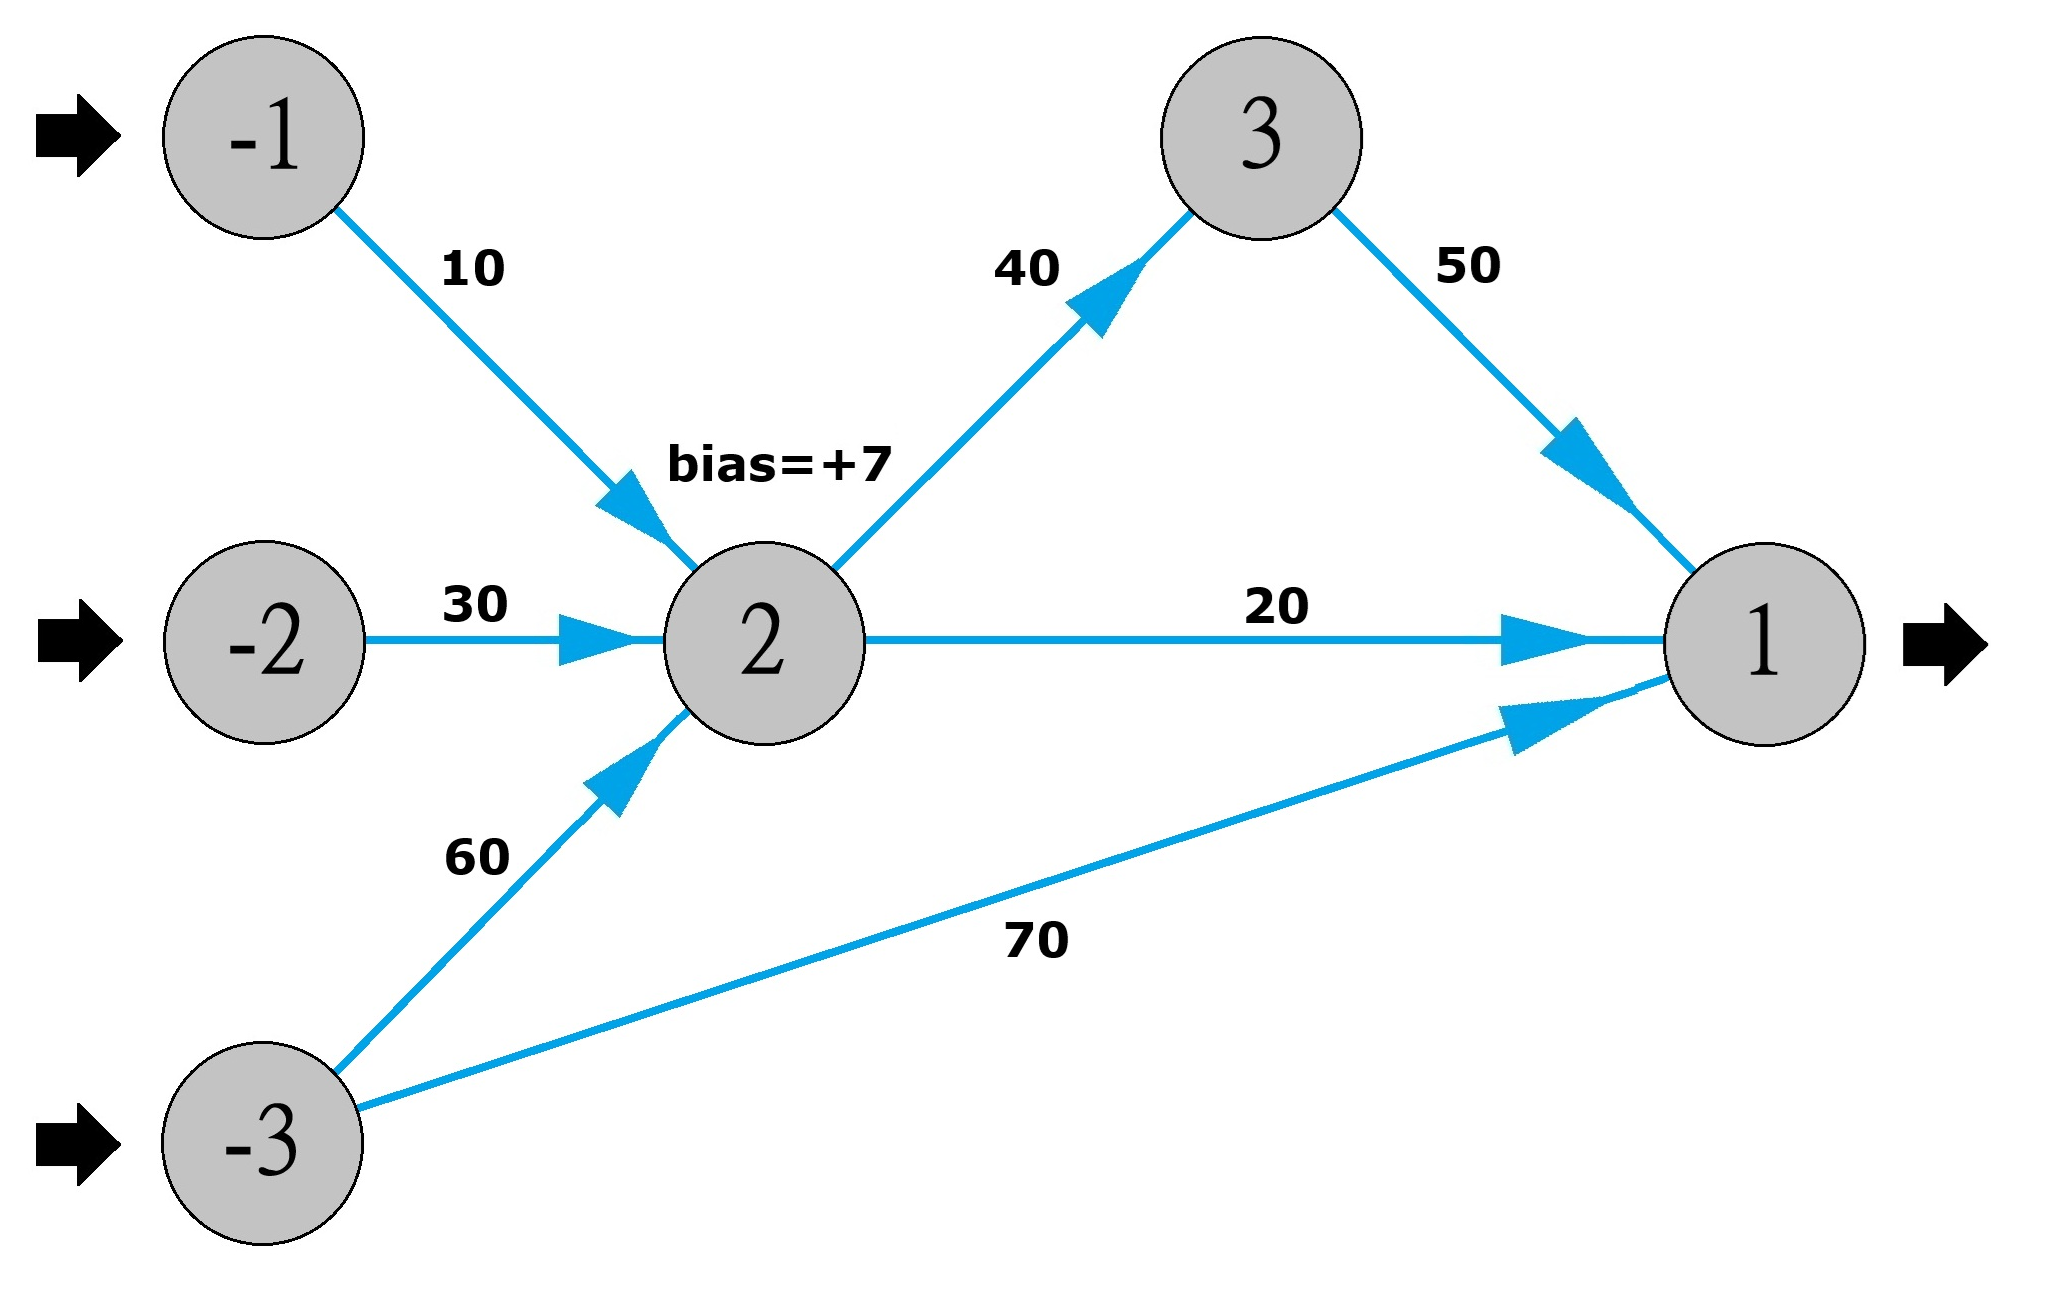
\includegraphics[width=0.64\textwidth]{img/neat-ncl/dynamic-nn-on-gpu/neat_ncl_dynamic_nn_on_gpu_example_1.png}
    \caption{An example NEAT dynamic neural network with connection weights and node bias labelled}
    \label{fig:neat_ncl_dynamic_nn_on_gpu_example_1}
\end{figure}


% 2 Image
\begin{figure}[H]
    \centering

    \begin{minipage}[t]{0.48\textwidth}
        \capstart
        \vspace{0pt}
        \centering
        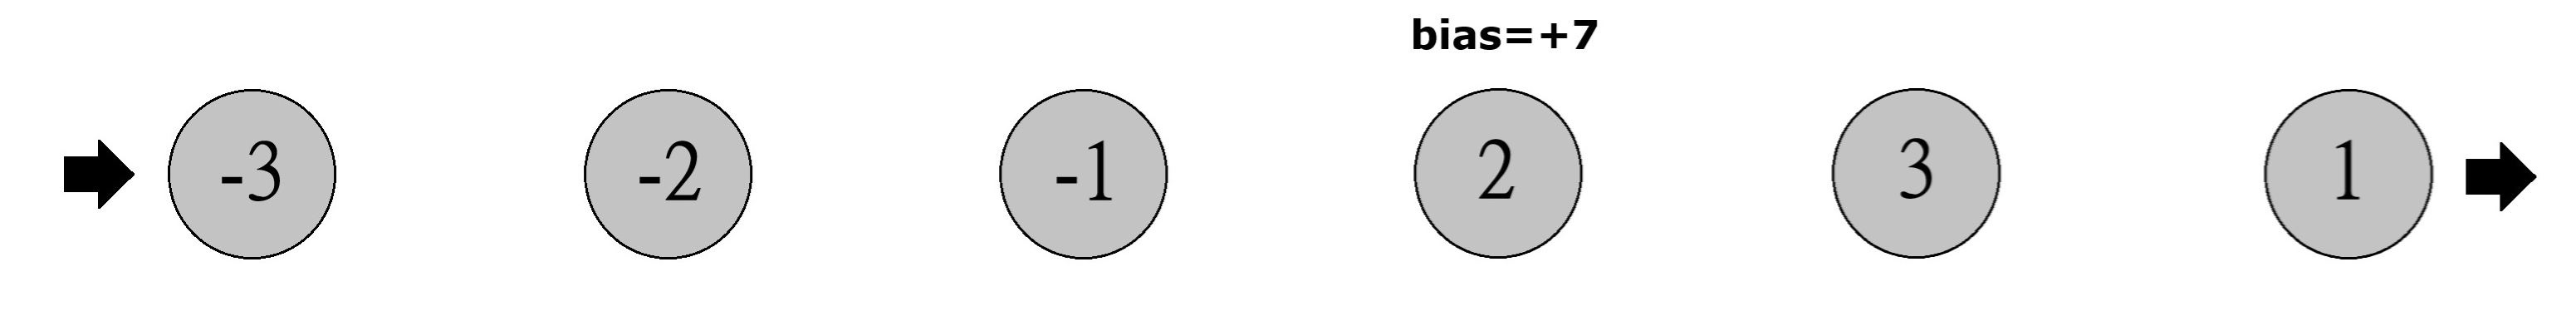
\includegraphics[width=\linewidth]{img/neat-ncl/dynamic-nn-on-gpu/neat_ncl_dynamic_nn_on_gpu_example_2.png}
        \caption{Compute the topological sort of nodes (read from left to right). }
        \label{fig:neat_ncl_dynamic_nn_on_gpu_example_2}
    \end{minipage}
    \hfill
    \begin{minipage}[t]{0.48\textwidth}
        \capstart
        \vspace{0pt}
        \centering
        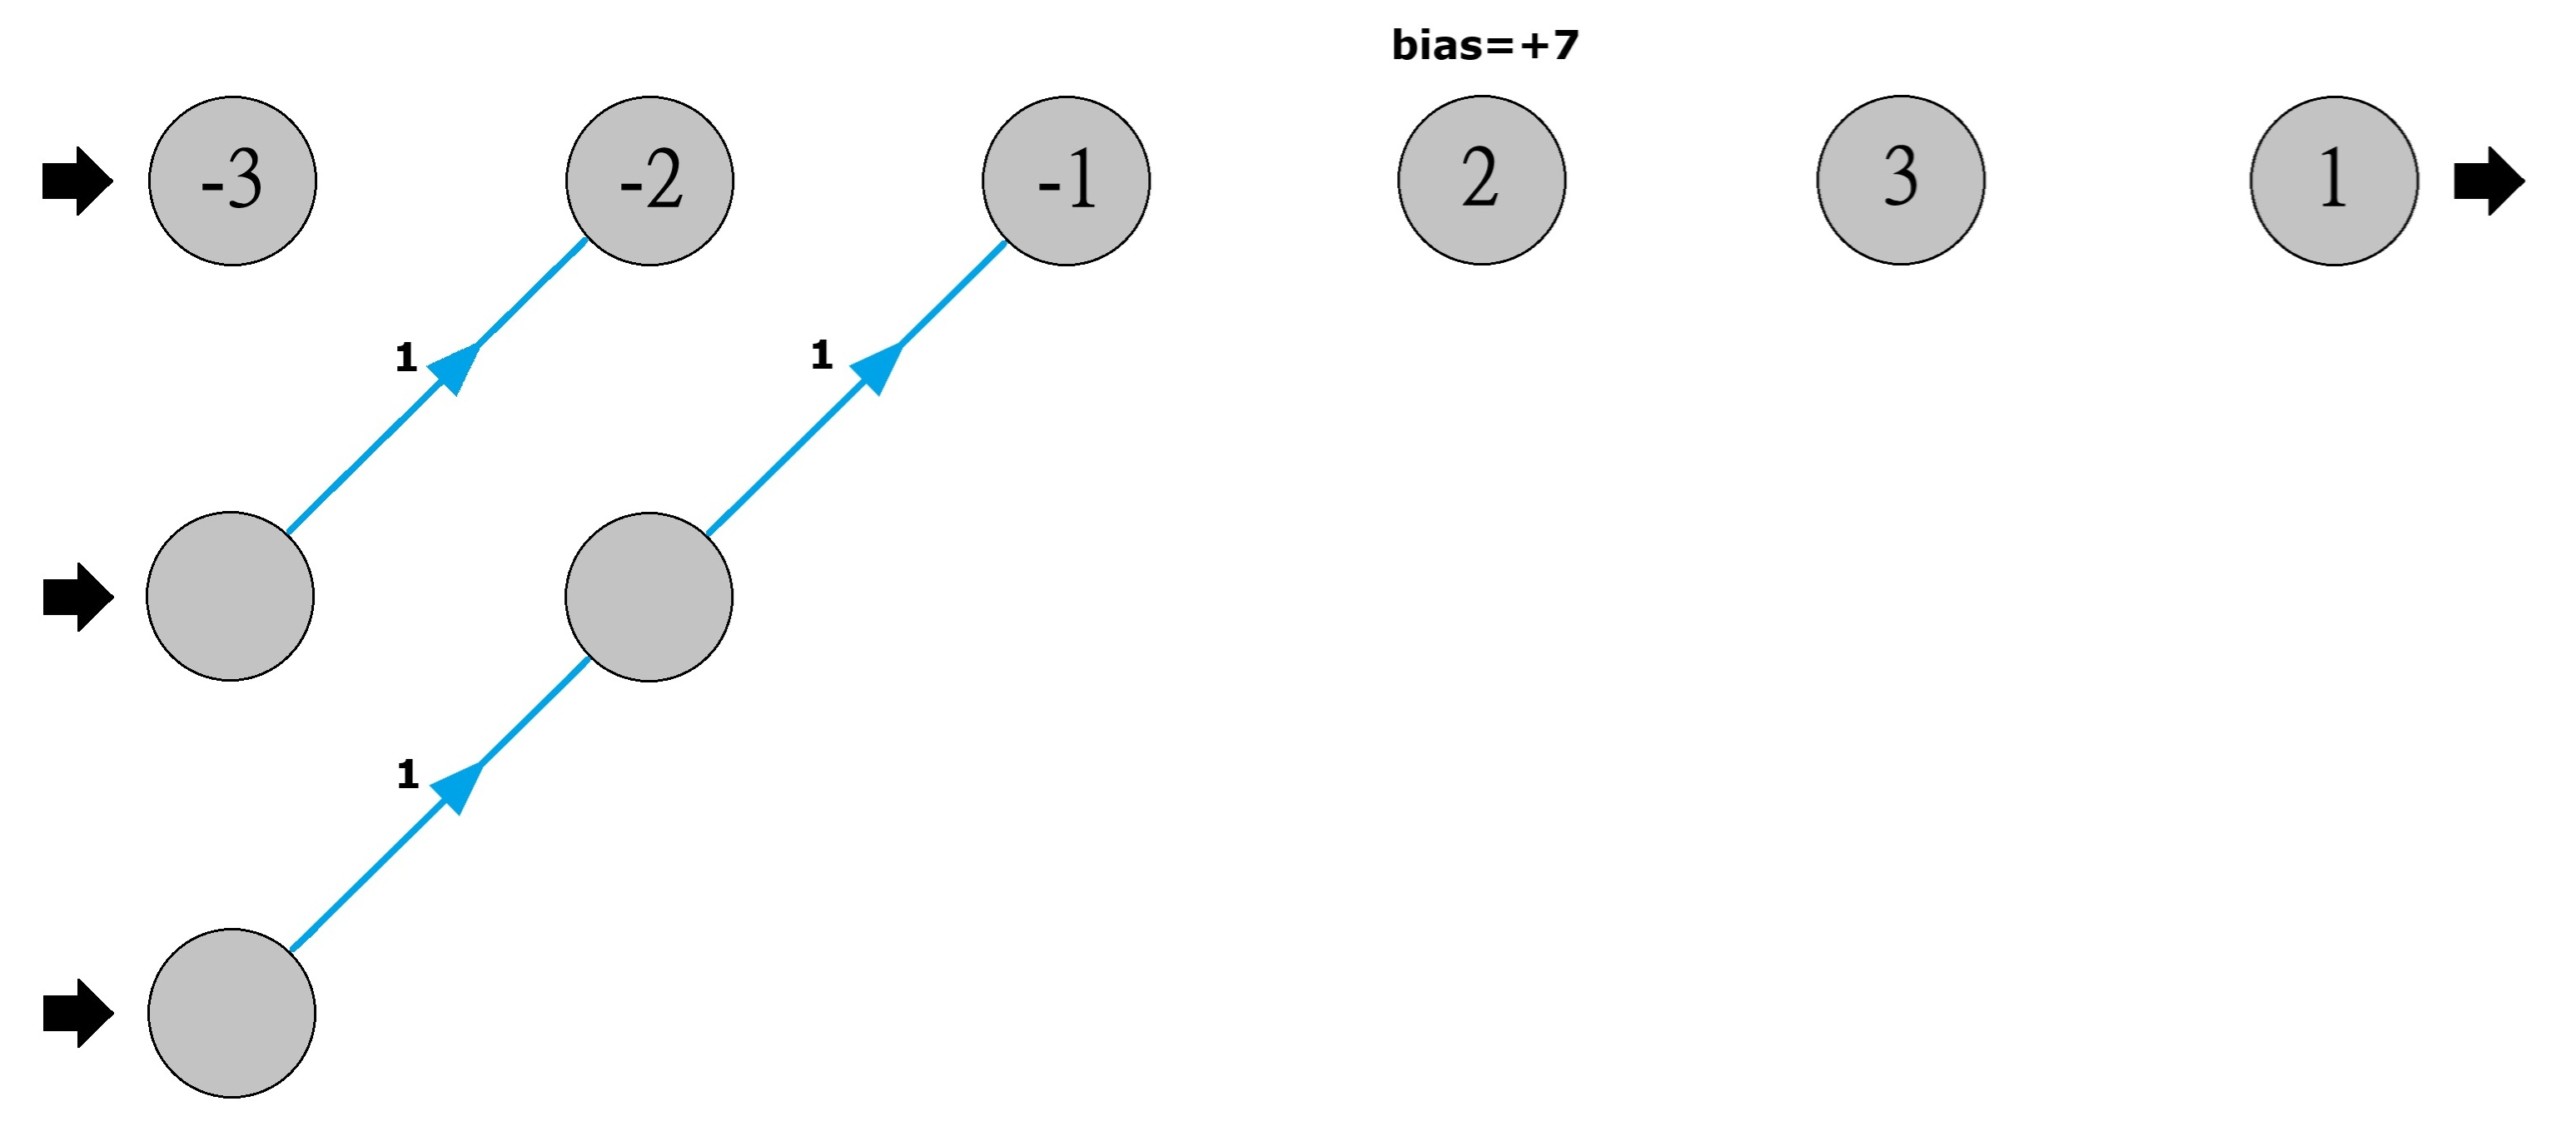
\includegraphics[width=\linewidth]{img/neat-ncl/dynamic-nn-on-gpu/neat_ncl_dynamic_nn_on_gpu_example_3.png}
        \caption{Connect all input neurons to the first layer directly. }
        \label{fig:neat_ncl_dynamic_nn_on_gpu_example_3}
    \end{minipage}
\end{figure}


% 2 Image
\begin{figure}[H]
    \centering

    \begin{minipage}[t]{0.48\textwidth}
        \capstart
        \vspace{0pt}
        \centering
        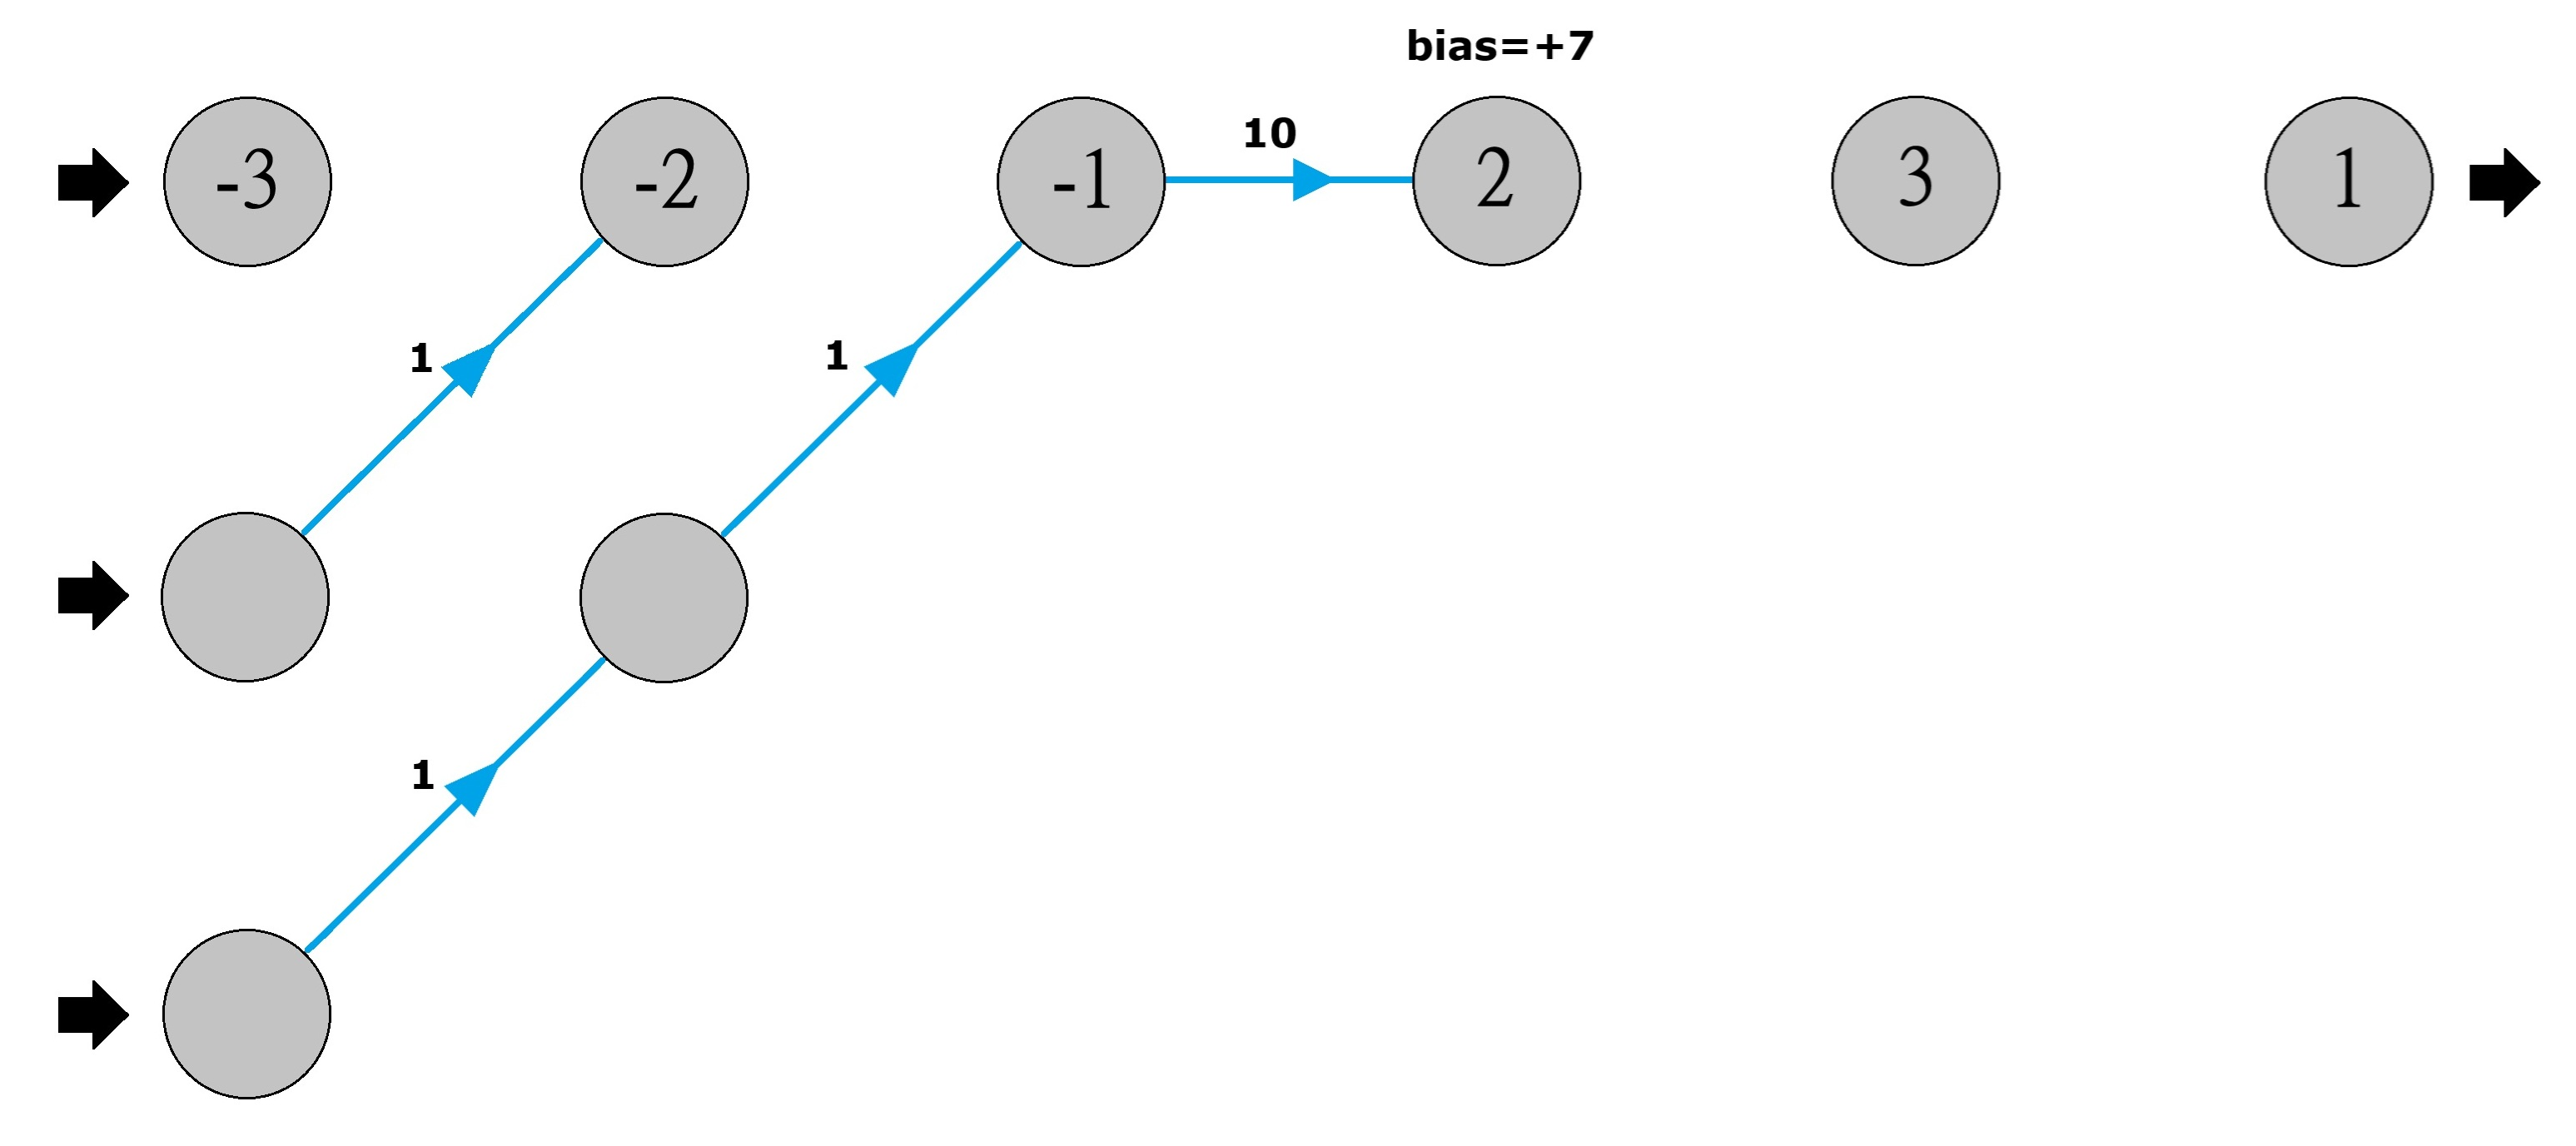
\includegraphics[width=\linewidth]{img/neat-ncl/dynamic-nn-on-gpu/neat_ncl_dynamic_nn_on_gpu_example_4.png}
        \caption{New connections and nodes are added to represent the connection \texttt{(-1, 2)} in the original DAG. }
        \label{fig:neat_ncl_dynamic_nn_on_gpu_example_4}
    \end{minipage}
    \hfill
    \begin{minipage}[t]{0.48\textwidth}
        \capstart
        \vspace{0pt}
        \centering
        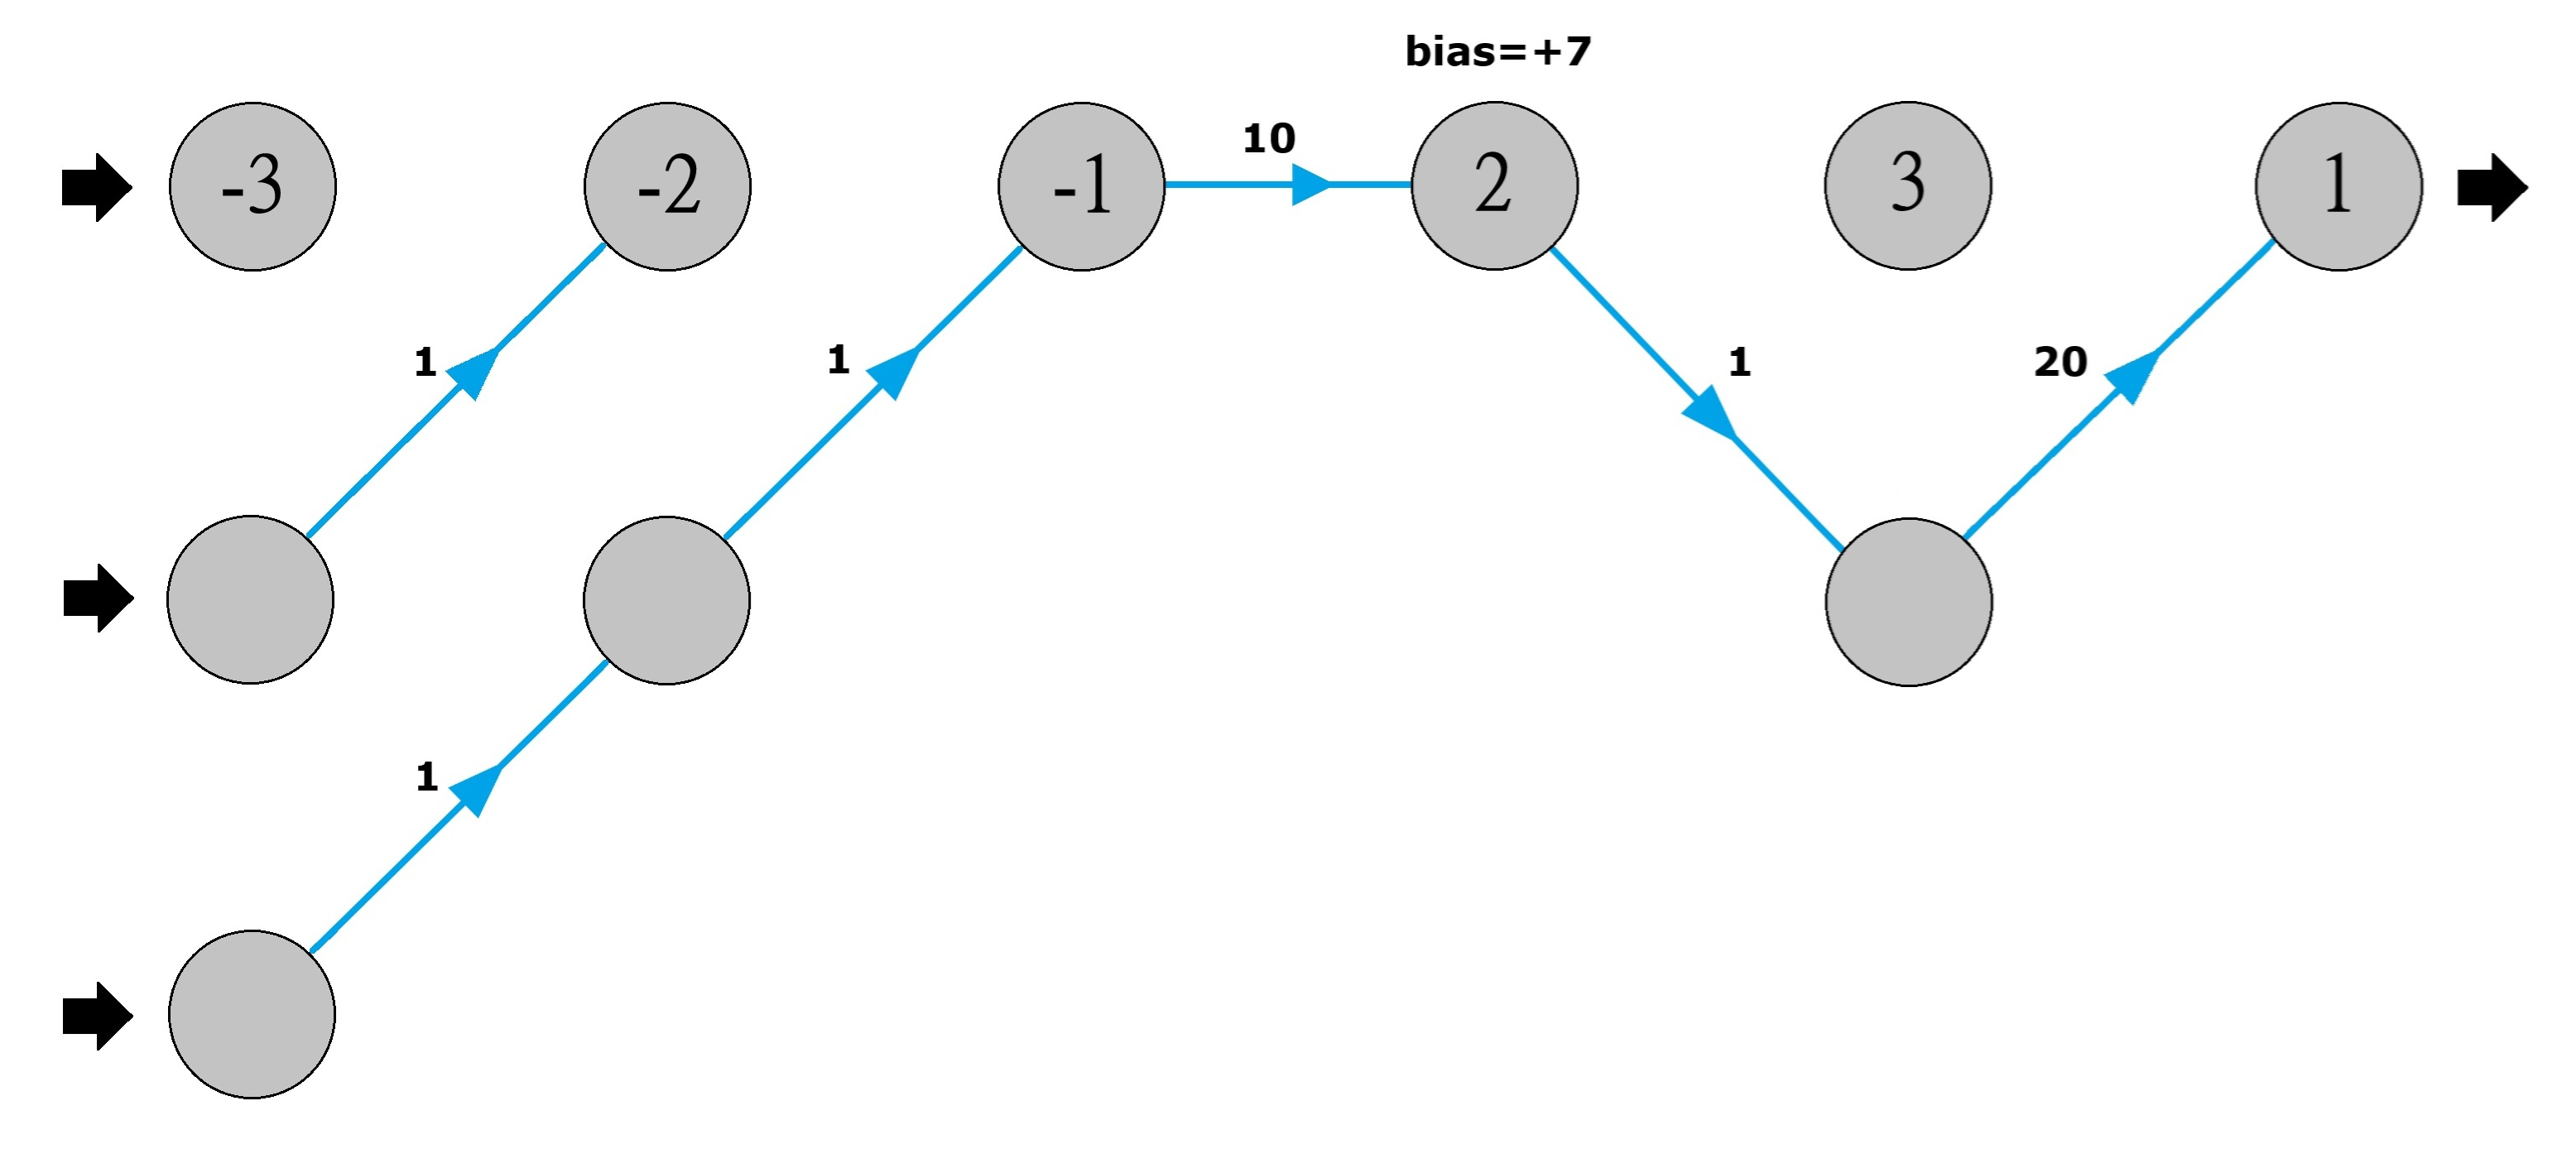
\includegraphics[width=\linewidth]{img/neat-ncl/dynamic-nn-on-gpu/neat_ncl_dynamic_nn_on_gpu_example_5.png}
        \caption{New connections and nodes are added to represent the connection \texttt{(2, 1)} in the original DAG. }
        \label{fig:neat_ncl_dynamic_nn_on_gpu_example_5}
    \end{minipage}
\end{figure}


% 2 Image
\begin{figure}[H]
    \centering

    \begin{minipage}[t]{0.48\textwidth}
        \capstart
        \vspace{0pt}
        \centering
        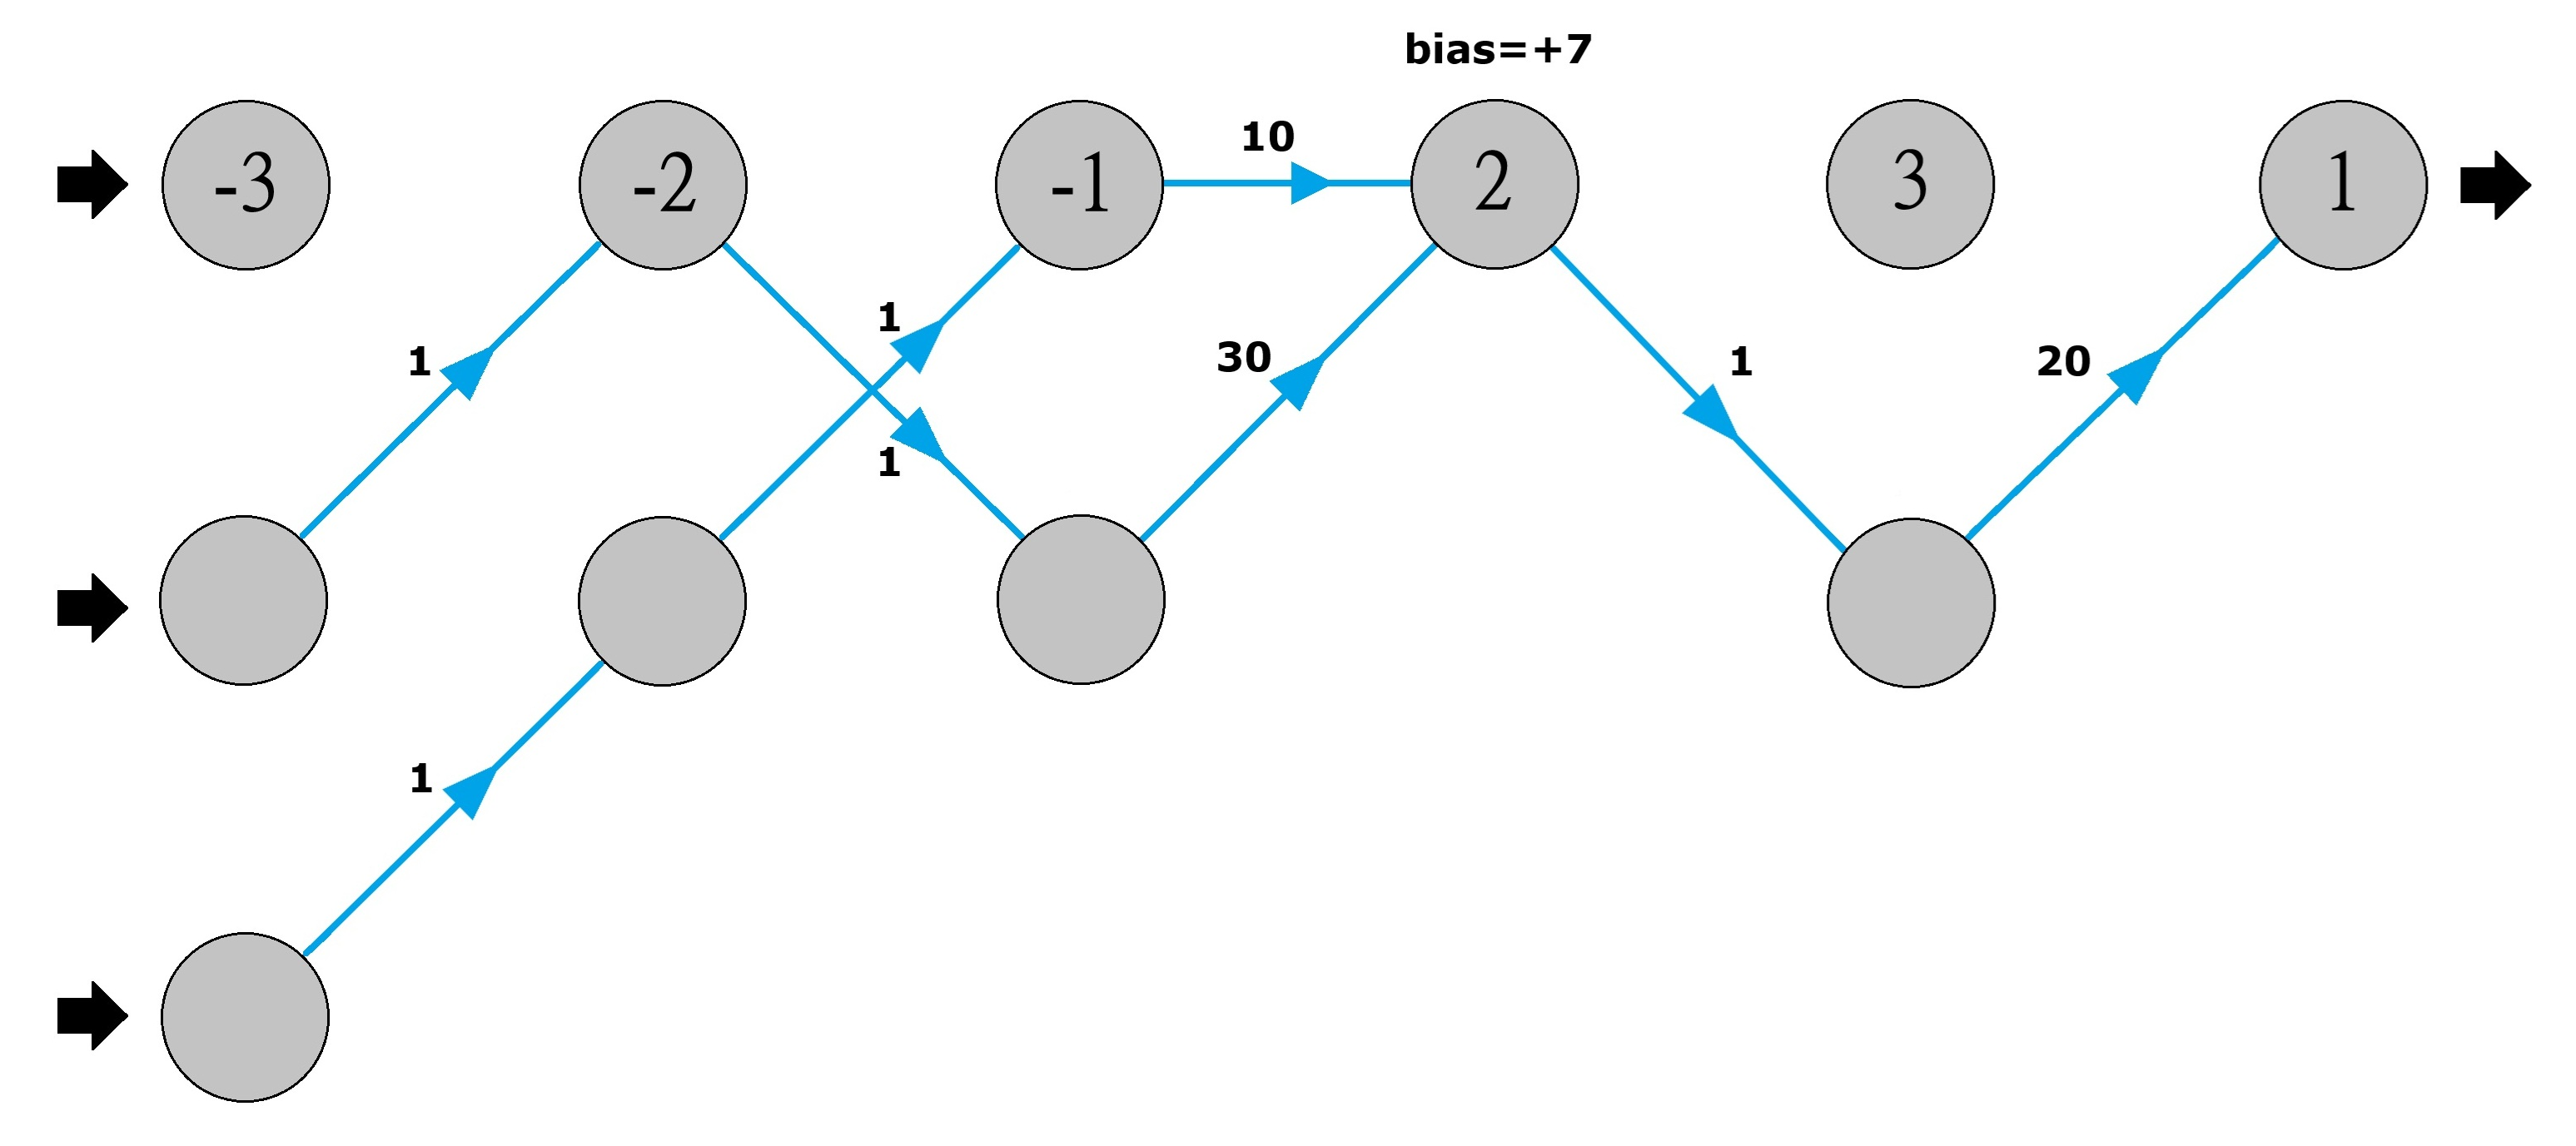
\includegraphics[width=\linewidth]{img/neat-ncl/dynamic-nn-on-gpu/neat_ncl_dynamic_nn_on_gpu_example_6.png}
        \caption{New connections and nodes are added to represent the connection \texttt{(-2, 2)} in the original DAG. }
        \label{fig:neat_ncl_dynamic_nn_on_gpu_example_6}
    \end{minipage}
    \hfill
    \begin{minipage}[t]{0.48\textwidth}
        \capstart
        \vspace{0pt}
        \centering
        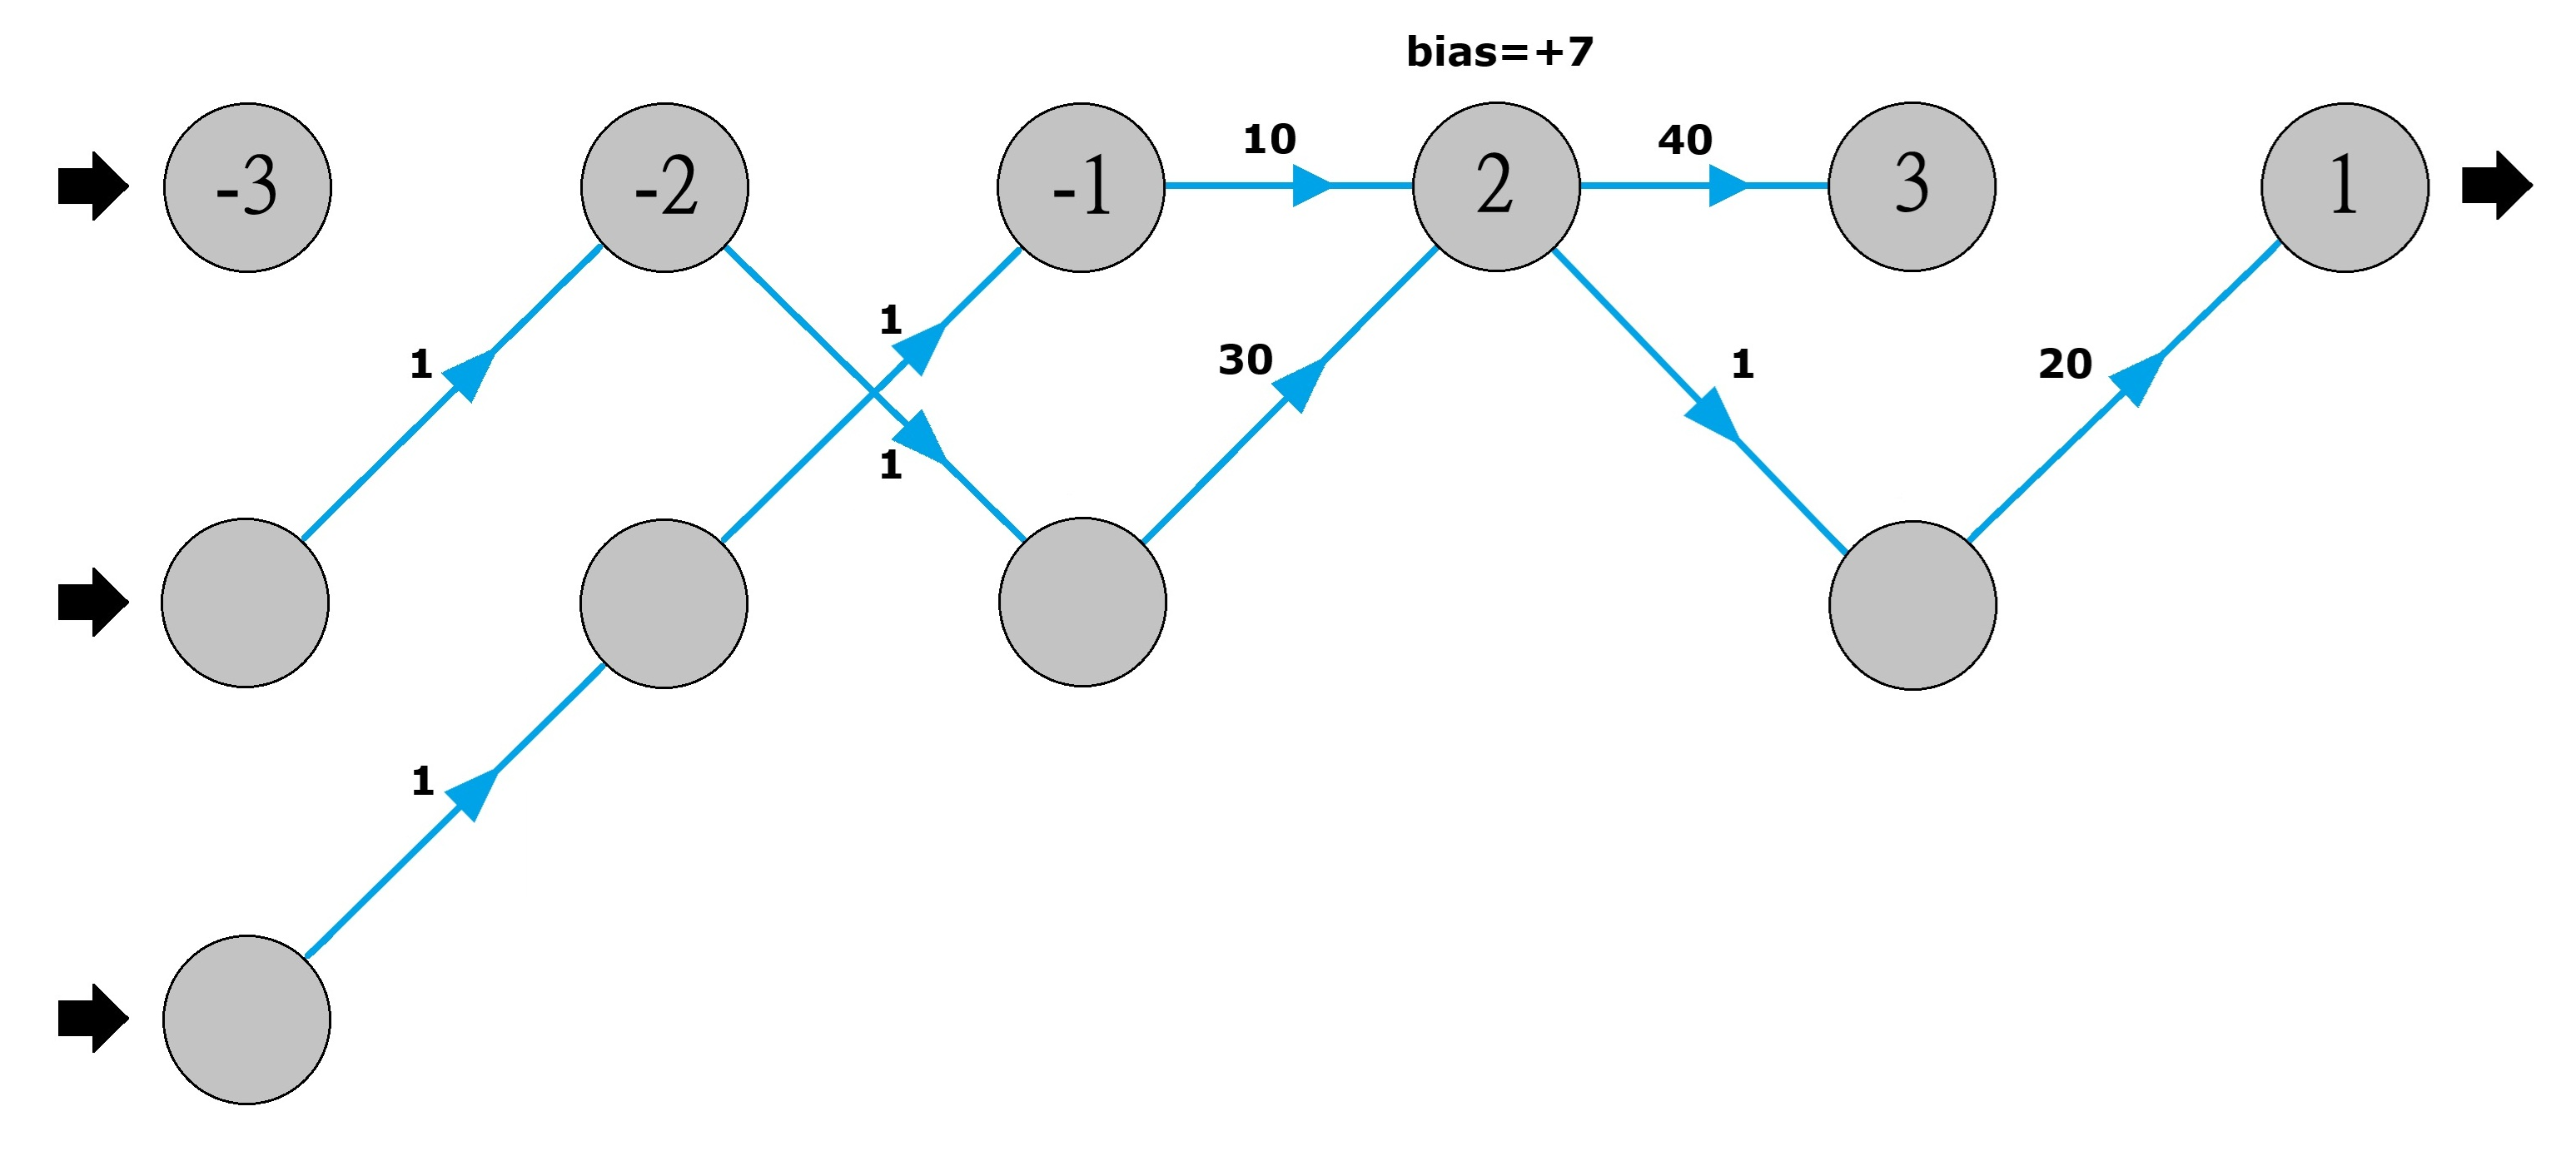
\includegraphics[width=\linewidth]{img/neat-ncl/dynamic-nn-on-gpu/neat_ncl_dynamic_nn_on_gpu_example_7.png}
        \caption{New connections and nodes are added to represent the connection \texttt{(2, 3)} in the original DAG. }
        \label{fig:neat_ncl_dynamic_nn_on_gpu_example_7}
    \end{minipage}
\end{figure}


% 2 Image
\begin{figure}[H]
    \centering

    \begin{minipage}[t]{0.48\textwidth}
        \capstart
        \vspace{0pt}
        \centering
        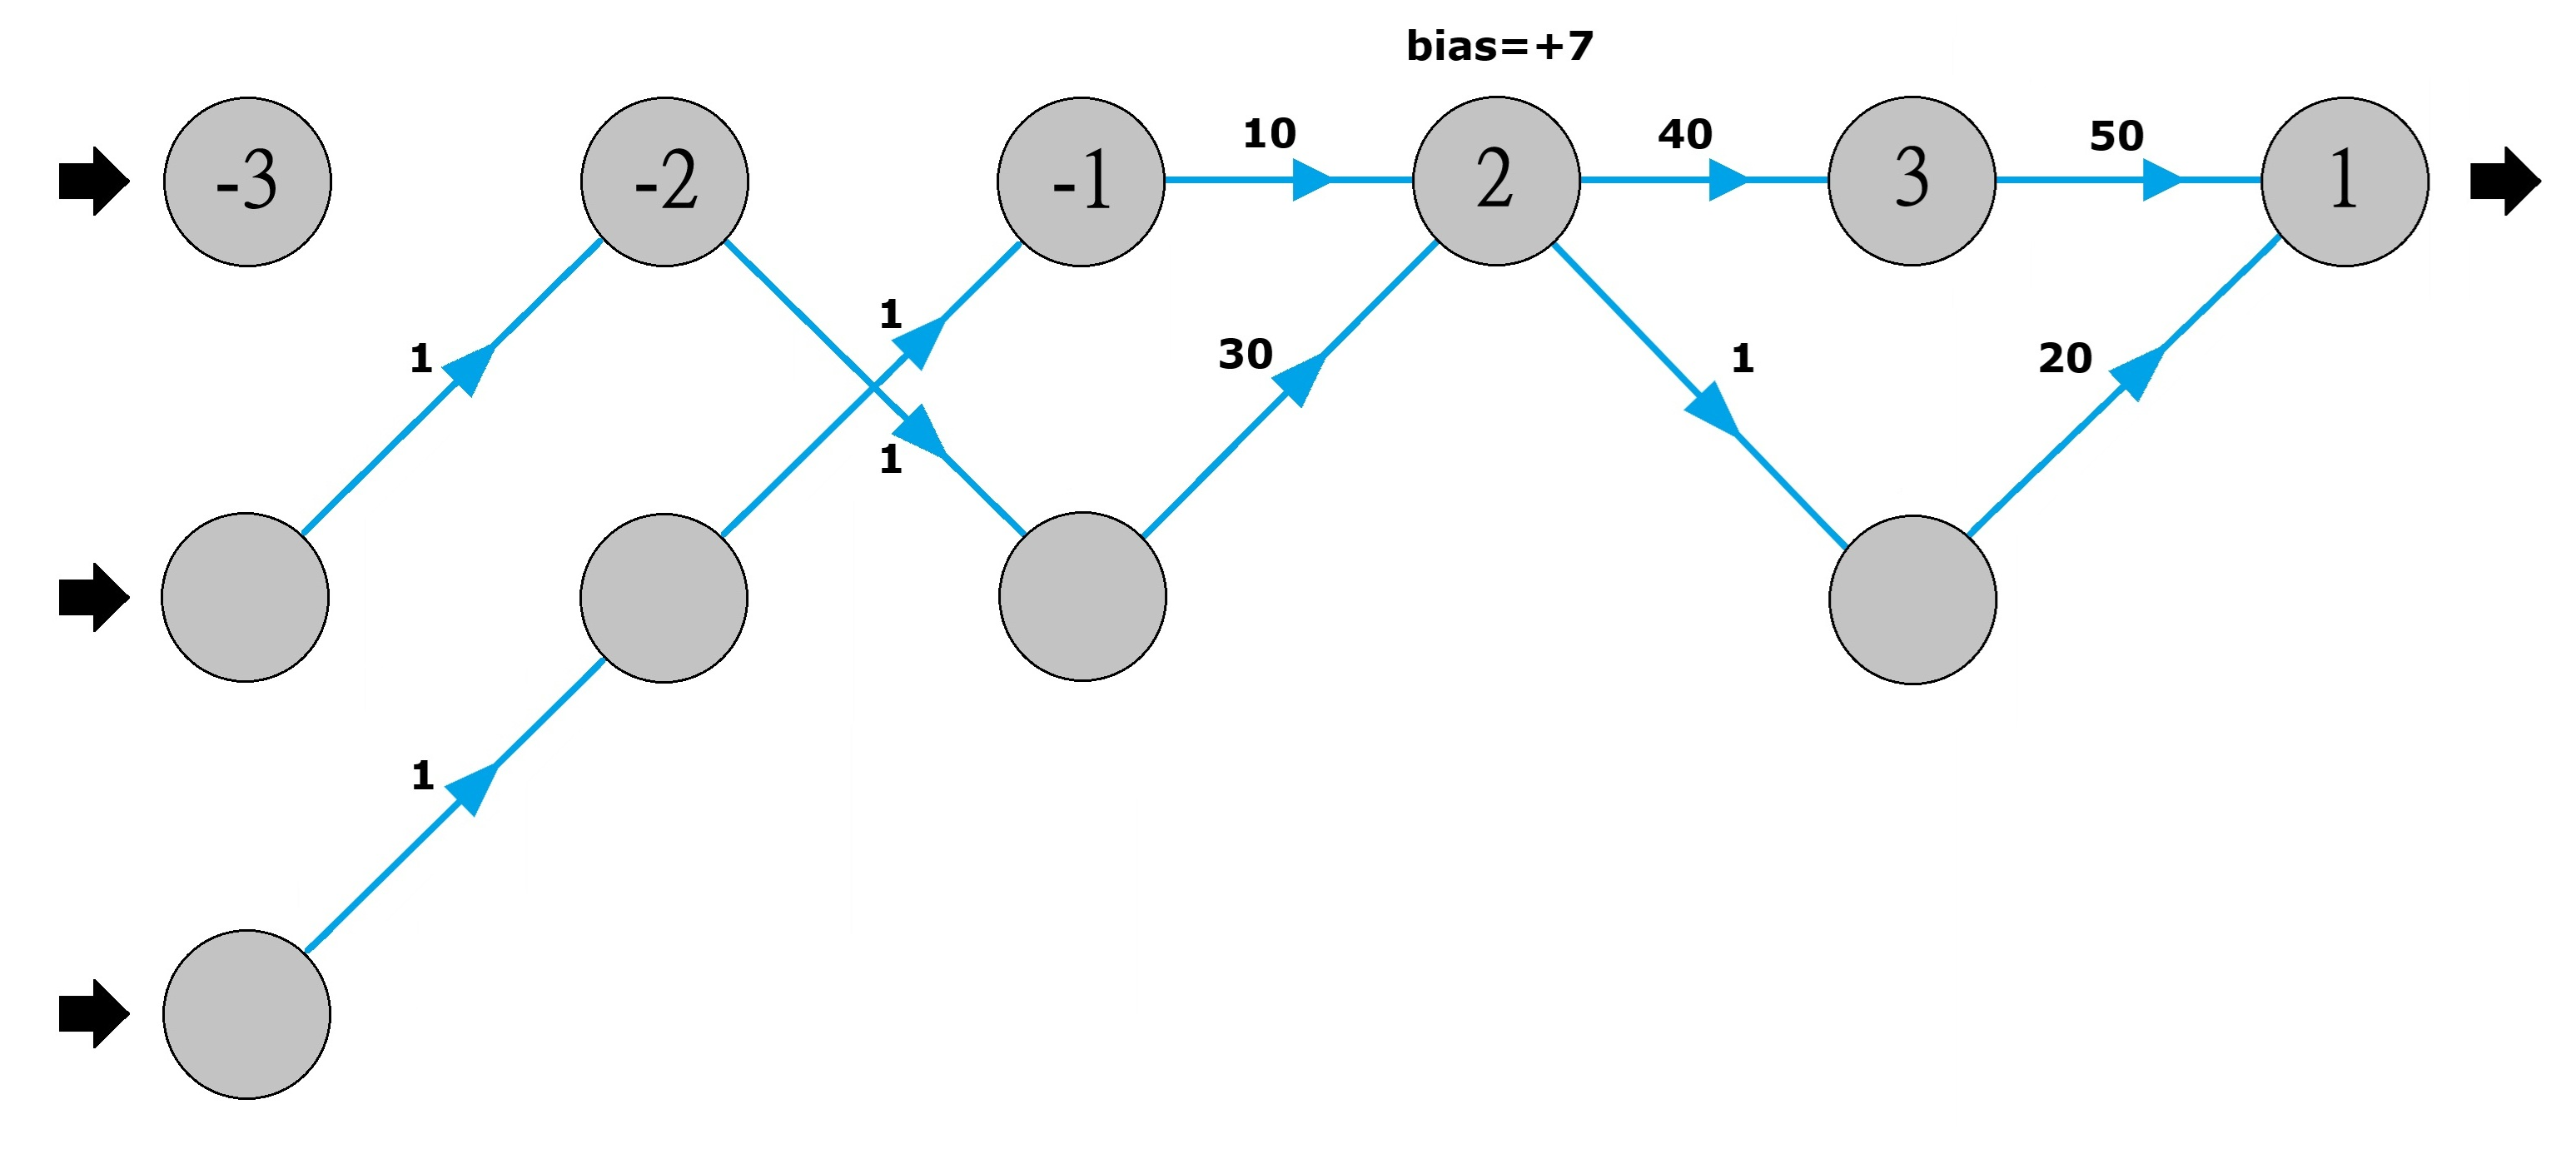
\includegraphics[width=\linewidth]{img/neat-ncl/dynamic-nn-on-gpu/neat_ncl_dynamic_nn_on_gpu_example_8.png}
        \caption{New connections and nodes are added to represent the connection \texttt{(3, 1)} in the original DAG. }
        \label{fig:neat_ncl_dynamic_nn_on_gpu_example_8}
    \end{minipage}
    \hfill
    \begin{minipage}[t]{0.48\textwidth}
        \capstart
        \vspace{0pt}
        \centering
        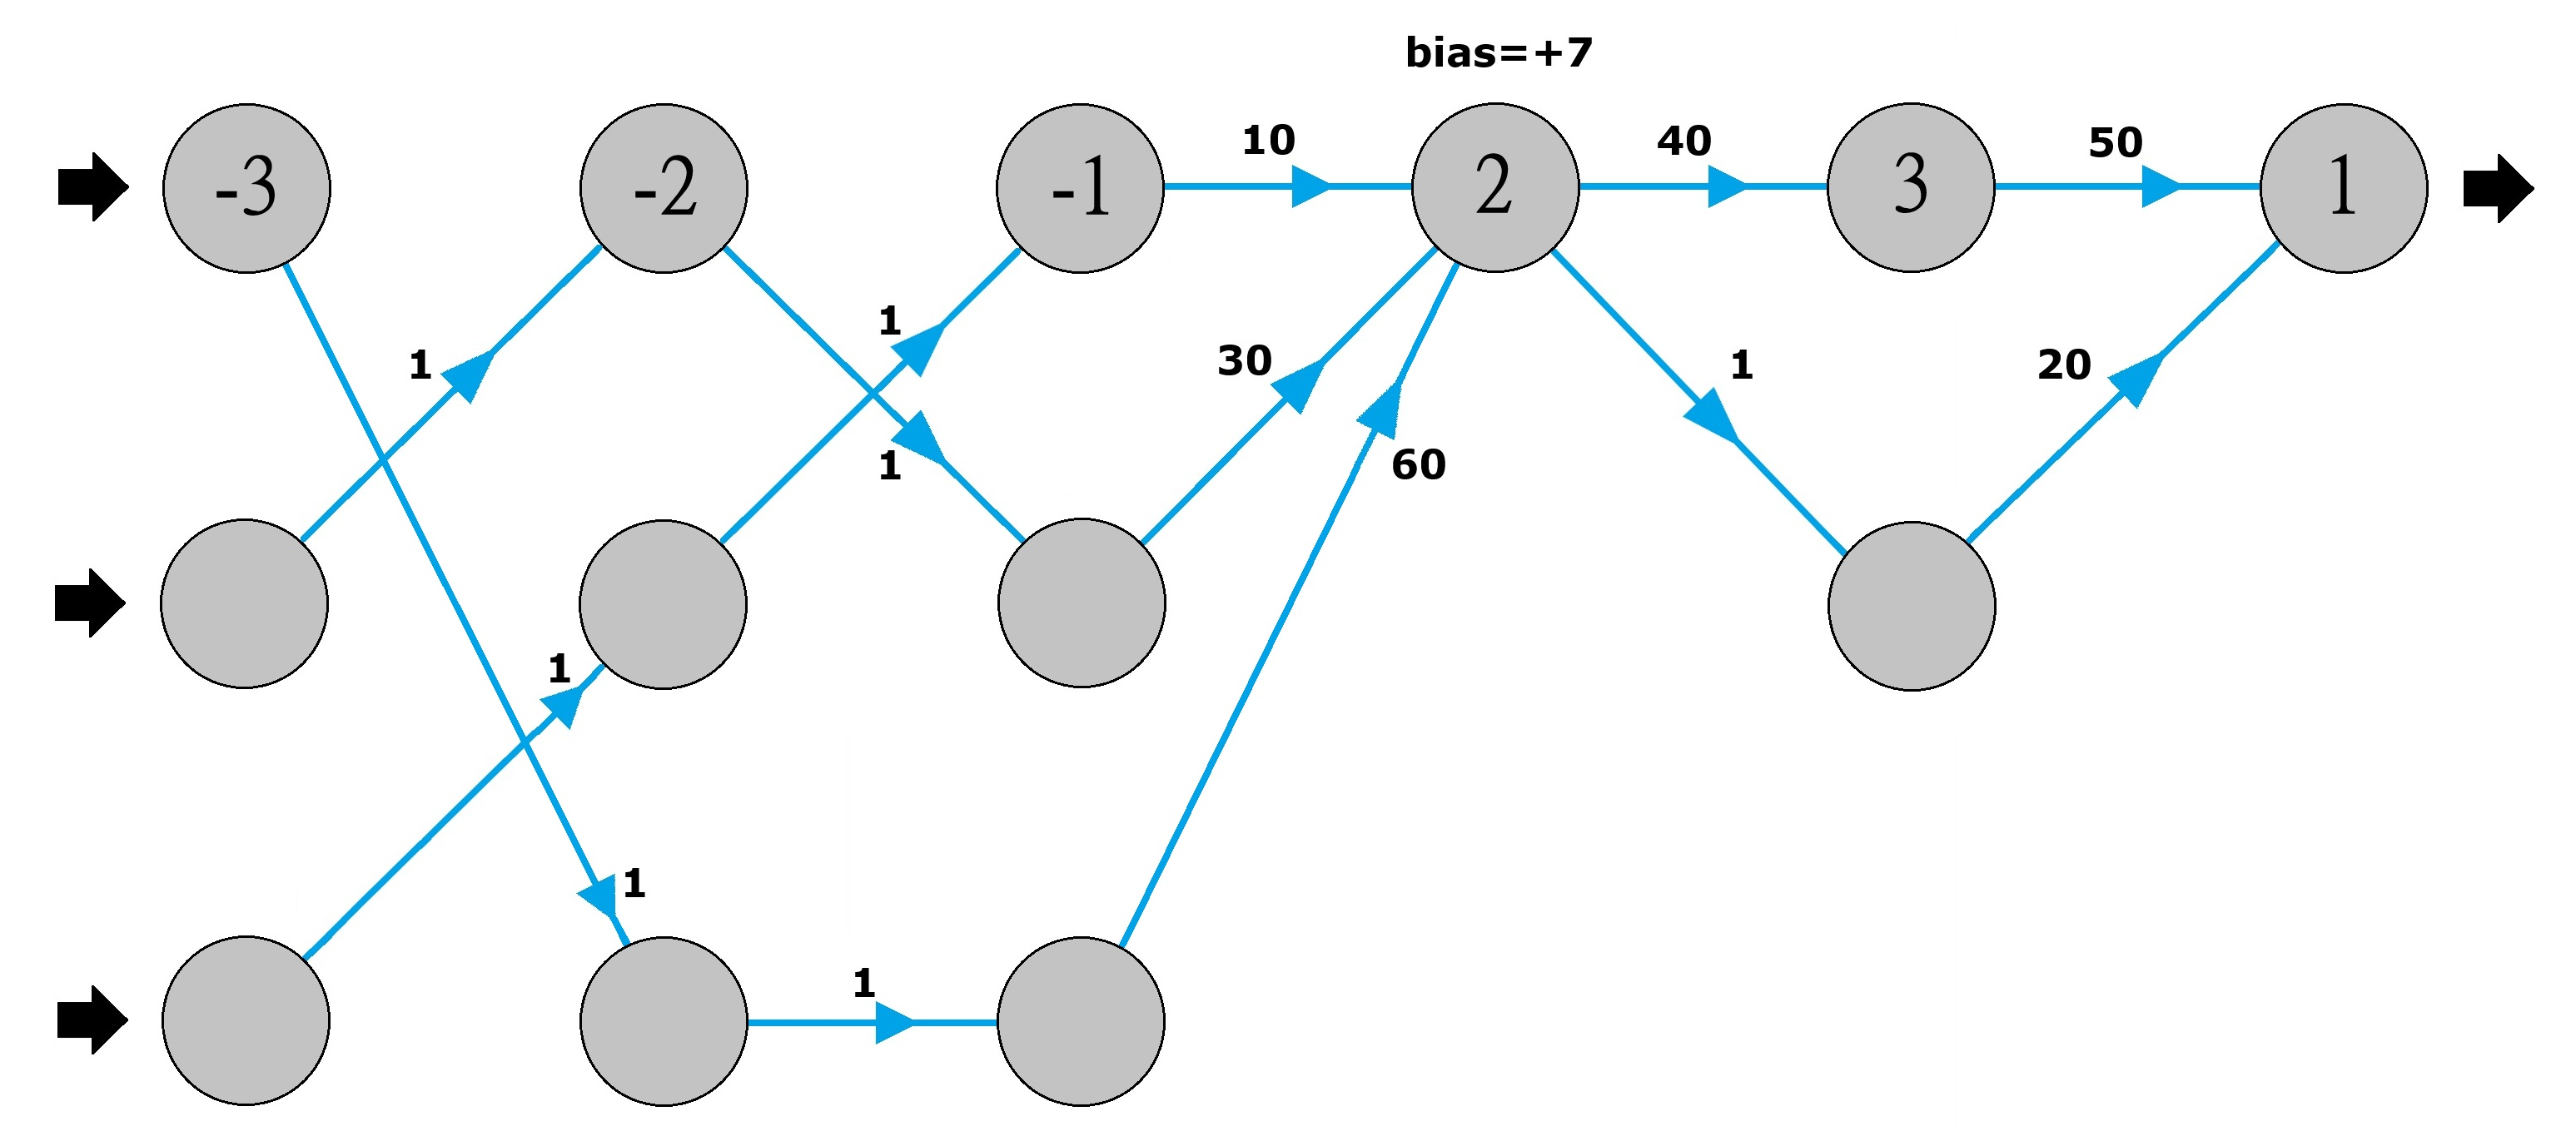
\includegraphics[width=\linewidth]{img/neat-ncl/dynamic-nn-on-gpu/neat_ncl_dynamic_nn_on_gpu_example_9.png}
        \caption{New connections and nodes are added to represent the connection \texttt{(-3, 2)} in the original DAG. }
        \label{fig:neat_ncl_dynamic_nn_on_gpu_example_9}
    \end{minipage}
\end{figure}


% 2 Image
\begin{figure}[H]
    \centering

    \begin{minipage}[t]{0.48\textwidth}
        \capstart
        \vspace{0pt}
        \centering
        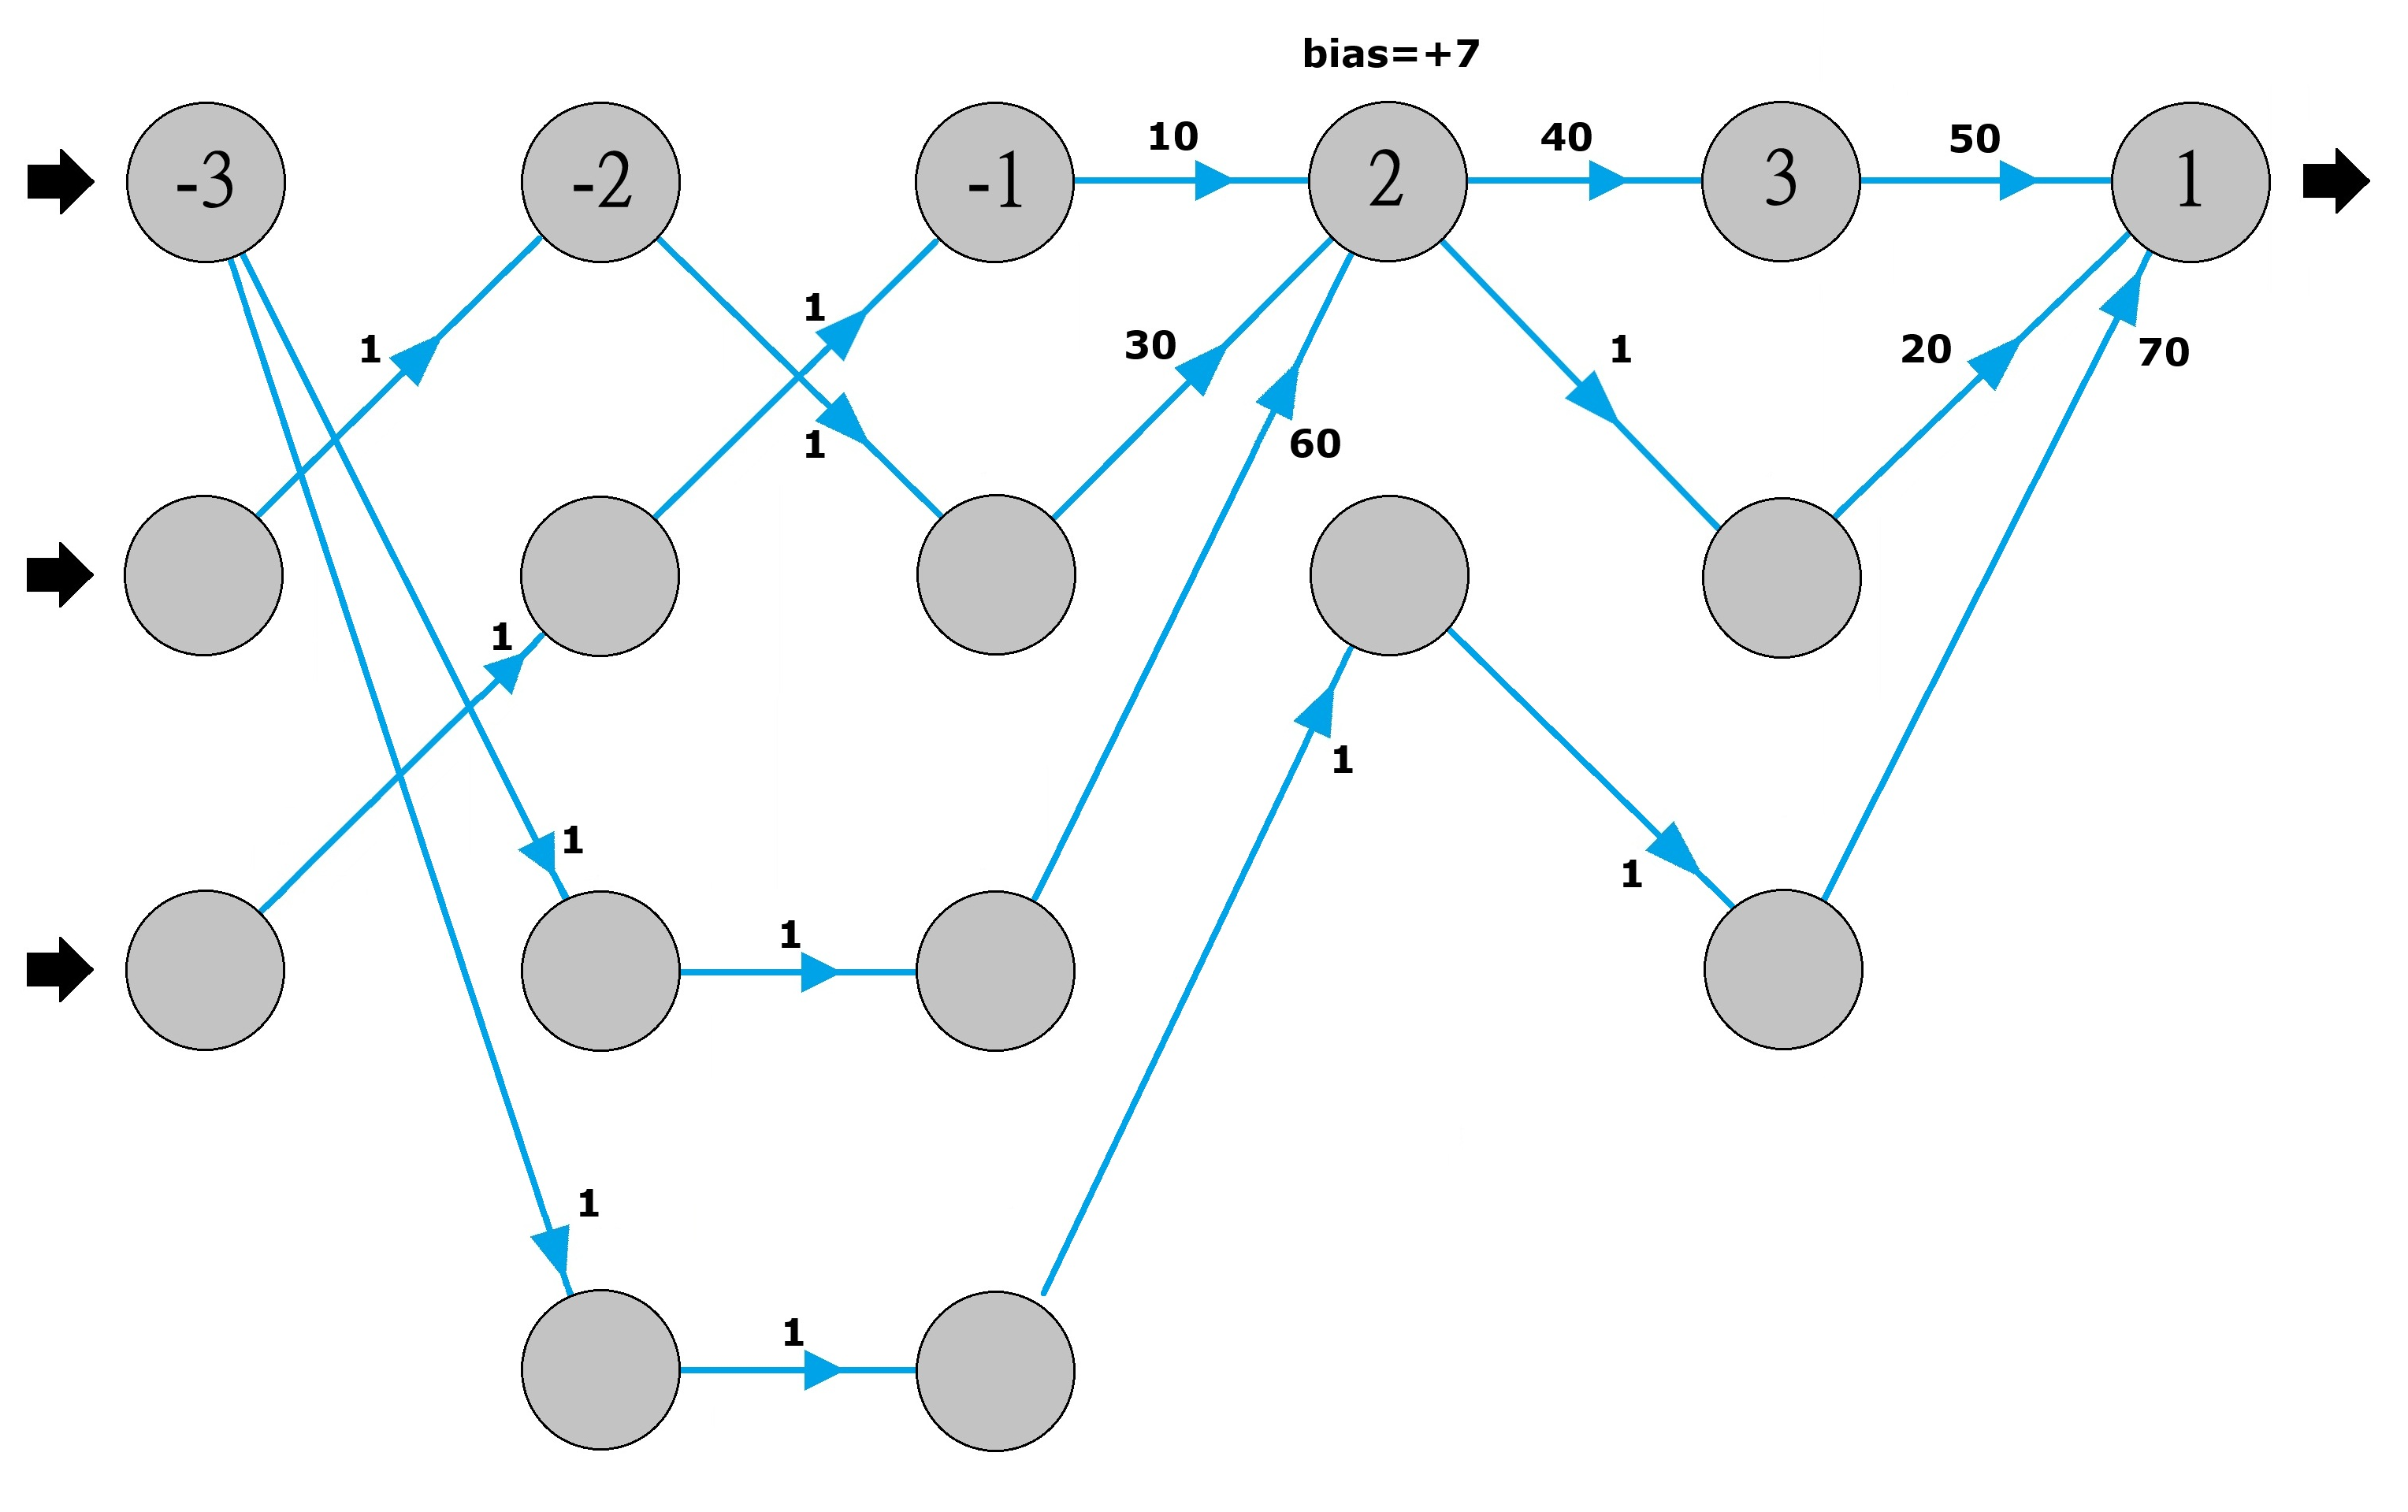
\includegraphics[width=\linewidth]{img/neat-ncl/dynamic-nn-on-gpu/neat_ncl_dynamic_nn_on_gpu_example_10.png}
        \caption{New connections and nodes are added to represent the connection \texttt{(-3, 1)} in the original DAG. The current graph is already an equivalent minimum graph of the original DAG but it is not enough to create the corresponding PyTorch MLP yet. }
        \label{fig:neat_ncl_dynamic_nn_on_gpu_example_10}
    \end{minipage}
    \hfill
    \begin{minipage}[t]{0.48\textwidth}
        \capstart
        \vspace{0pt}
        \centering
        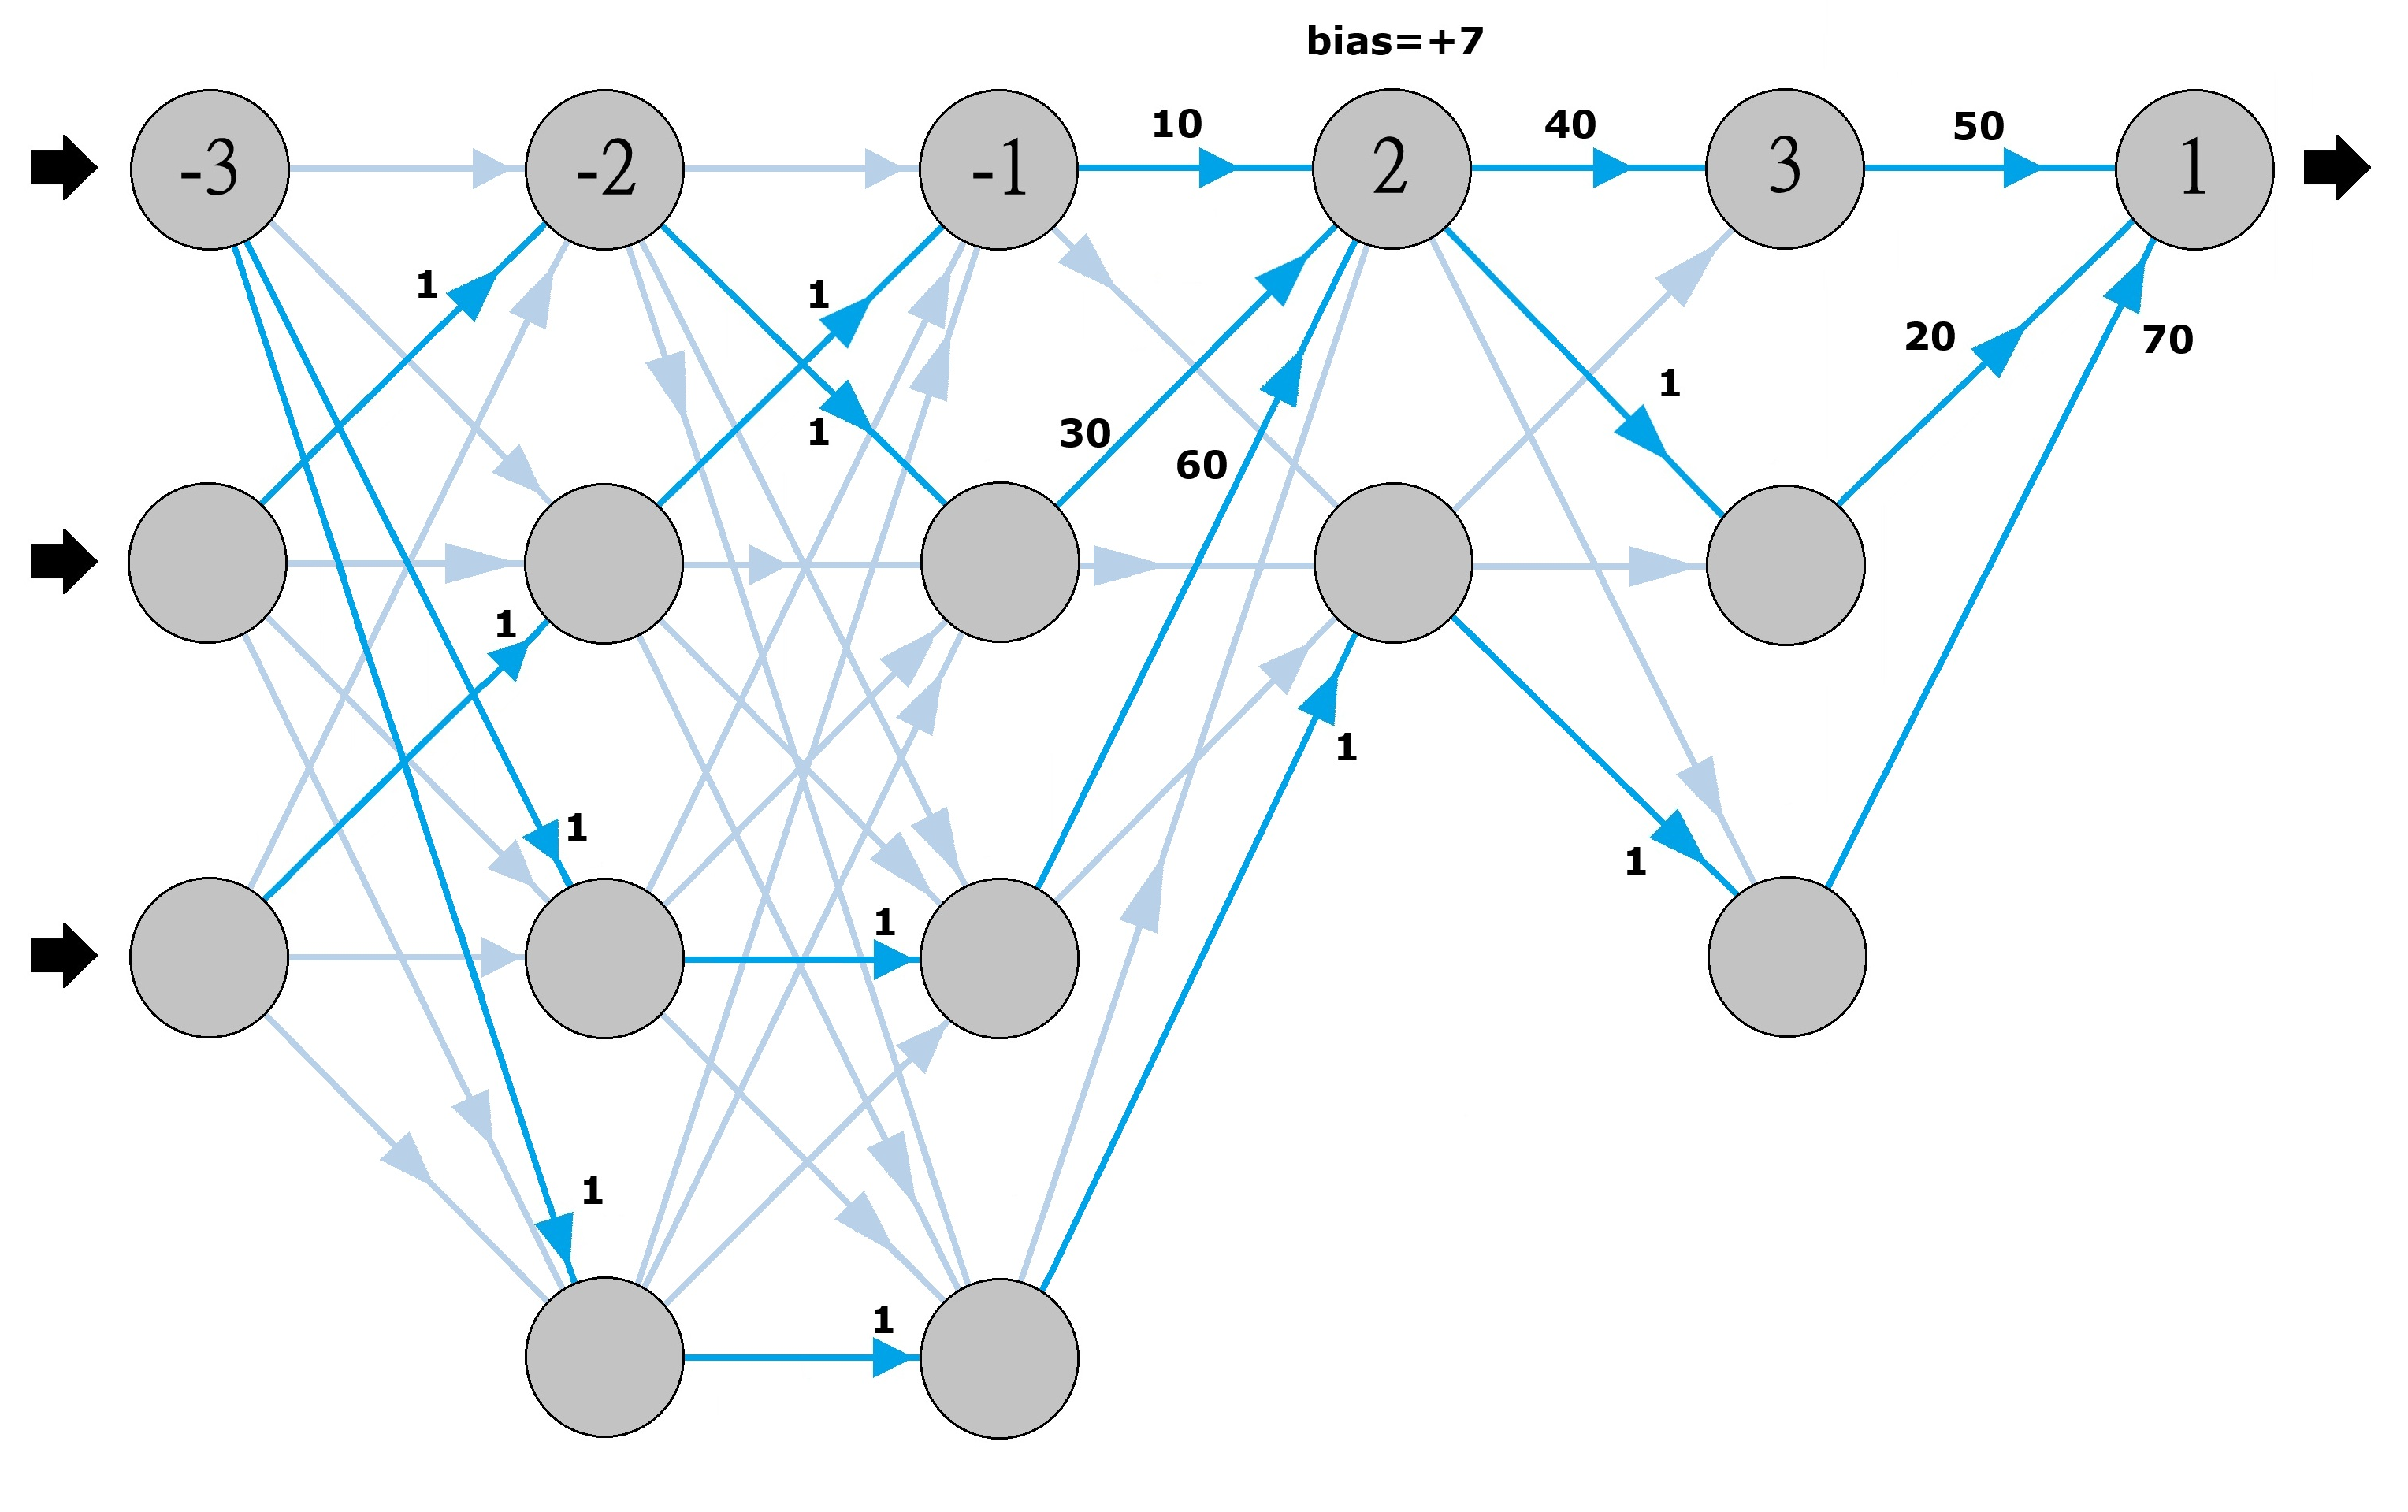
\includegraphics[width=\linewidth]{img/neat-ncl/dynamic-nn-on-gpu/neat_ncl_dynamic_nn_on_gpu_example_11.png}
        \caption{Add connections with weight~$0$ to make the network fully-connected. The translucent connections have weight~$0$ while the solid connections have weights other than $0$. }
        \label{fig:neat_ncl_dynamic_nn_on_gpu_example_11}
    \end{minipage}
\end{figure}


\paragraph{Experimental Design}
Experiments had been conducted to compare the performance of a NEAT-NCL model with a control arithmetic-mean-ensemble, a control NCL model and a control MLP. Table~\ref{table:experiment_4_varied_hyperparameters} contains all varied hyperparameters. Table~\ref{table:experiment_4_fixed_hyperparameters} contains all fixed hyperparameters. Table~\ref{table:experiment_4_metric} contains all evaluation metrics collected in this experiment. For raw fitness and adjusted fitness, the larger their values, the better the genome is. 

\begin{table}[H]
    \centering
    \begin{tabular}{|c|c|c|c|}
        \hline
        Hyperparameter & Type & Choices / Ranges & Description \\
        \hline
        \small\texttt{ensemble\_sizes} & Integer & $[50, 250]\text{, step}=50$ & $m$ \\
        \hline
    \end{tabular}
    \caption{Varied hyperparameters and their configurations}
    \label{table:experiment_4_varied_hyperparameters}
\end{table}

\begin{table}[H]
    \centering
    \begin{tabular}{|c|c|c|p{5cm}|}
        \hline
        Hyperparameter & Type & Choices / Ranges & Description \\
        \hline
        \small\texttt{input\_size} & Integer & $13$ & Number of input features of the MLP \\
        \hline
        \small\texttt{output\_size} & Integer & $1$ & Number of labels of the MLP \\
        \hline
        \small\texttt{optimizer} & Categorical & \texttt{torch.optim.Adam} & Optimisation algorithm used for training \\
        \hline
        \small\texttt{learning\_rate} & Float & $0.001$ & Learning rate of the optimisation algorithm \\
        \hline
        \small\texttt{activation} & Categorical & ReLU & Activation function used in each dense layer of the MLP \\
        \hline
        \small\texttt{evolution\_epoch} & Integer & \{$500$\} & Number of evolutionary generations during training \\
        \hline
        \small\texttt{voter} & Categorical & \texttt{arithmetic\_mean} & Type of aggregator used to combine base learners' predictions \\
        \hline
        \small\texttt{min\_lambda} & Float & $0.1$ & $\lambda_{min}$ \\
        \hline
        \small\texttt{max\_lambda} & Float & $0.9$ & $\lambda_{max}$ \\
        \hline
        \small\texttt{evolution\_epoch\_step\_size} & Integer & $10$ & Number of evolutionary generations to collect all metrics once \\
        \hline
        \small\texttt{batch\_size} & Integer & $506$ & Number of training samples passed to phenomes in one go \\
        \hline
    \end{tabular}
    \caption{Fixed hyperparameters and their configurations}
    \label{table:experiment_4_fixed_hyperparameters}
\end{table}

\begin{table}[H]
    \centering
    \begin{tabular}{|c|c|p{5cm}|}
        \hline
        Metric & Type & Description \\
        \hline
        \small\texttt{loss\_test} & Float & MSE of ensemble model during testing \\
        \hline
        \small\texttt{average\_active\_hidden\_node\_num} & Float & Average number of active hidden nodes in a phenome during testing \\
        \hline
        \small\texttt{diversity\_coefficient\_test} & Float & $\rho$ during testing \\
        \hline
        \small\texttt{population\_diversity\_test} & Float & $D$ during testing \\
        \hline
        \small\texttt{max\_population\_diversity\_test} & Float & $D_{max}$ during testing \\
        \hline
        \small\texttt{correlation\_penalty\_coefficient\_test} & Float & $\lambda$ during testing \\
        \hline
        \small\texttt{subpopulation\_num} & Integer & Number of subpopulations during testing \\
        \hline
        \small\texttt{average\_niche\_radius} & Float & $\sigma$ during testing \\
        \hline
        \small\texttt{average\_sharing\_factor} & Float & Average sharing factor of all phenomes during testing \\
        \hline
        \small\texttt{average\_raw\_fitness} & Float & Average raw fitness of all phenomes during testing \\
        \hline
        \small\texttt{average\_adjusted\_fitness} & Float & Average adjusted fitness (after fitness sharing) of all phenomes during testing \\
        \hline
    \end{tabular}
    \caption{Evaluation metrics}
    \label{table:experiment_4_metric}
\end{table}


\paragraph{Reference Experiment}
The experiment on NEAT-NCL ensemble model was based on the NEAT-NCL experiments conducted in Sheng et al.\ \cite{sheng2017niching}. It aimed at reproducing similar experiment results to study the effect of NEAT-NCL on ensemble loss. To extend the experiment, three modifications had been added to the experiment in this work. 

In order to better compare the performance of NEAT-NCL ensemble model and the previous ensemble performance, MSE of a control MLP, an arithmetic-mean-ensemble (from Section~\ref{subsec:stage_2}) and a NCL ensemble model (from Section~\ref{subsec:stage_3}) had been added. Furthermore, the original experiment contained graphs of MSE, number of hidden nodes and population diversity $D$. To allow deeper analysis, more graphs had been added to this experiment, including raw fitness, adjusted fitness, sharing factor, $\sigma$, $\lambda$. Lastly, the formula of genetic distance for calculating the $D$ was modified. The modified formula has different weights for different types of genes and does not treat all connection weights equally. 


\subsection{Analyse Different Aggregators}
\label{subsec:stage_5}
\paragraph{Motivation}
In all previous designs, an arithmetic-mean-aggregator was used to combine predictions from base learners. Thus, every learner was treated with equal importance, contributing an identical weight to the final ensemble output. Beyond simple averaging, alternate aggregation strategies may offer improved robustness. For instance, a median-aggregator could better mitigate the impact of data skewness or outliers. Additionally, inspired by weighted majority voting~\cite{littlestone1994weighted}, we investigate the change in performance when base learners are assigned varying degrees of importance. These ideas correspond to the three respective, distinct aggregator types investigated in this stage: an arithmetic-mean-aggregator, a median-aggregator and a neural-network-aggregator. Note that when base learners are trained independently, using a neural-network-aggregator is equivalent to classical Stacking~\cite{wolpert1992stacked}~\cite{breiman1996stacked}. Furthermore, the results from this analysis also serve as a baseline for Section~\ref{subsec:stage_6}, where we investigate how specific ensemble architectures interact with different aggregation mechanisms. 

This brings us to the next stage of our analogy: how does the quality of a decision making change if certain company directors are given more voting power? 


\subsubsection{Updated NCL loss functions}
When a neural-network-aggregator is used, the loss function of a base learners is updated using the formula below: 
\begin{equation}
    \label{equation:recursive_nn_loss_function_base_learner}
    \mathcal{L}_i = (\hat{y}_i - y)^2 - \lambda (\hat{y}_i - \hat{y}_{ensemble})^2
\end{equation}
, where $\hat{y}_{ensemble}$ is the output of the neural-network-aggregator. When a neural-network-aggregator is used, the loss function of the neural-network-aggregator is updated using the formula below: 
\begin{equation}
    \label{equation:recursive_nn_loss_function_aggregator}
    \mathcal{L}_{ensemble} = (\hat{y}_{ensemble} - y)^2
\end{equation}
, where $\hat{y}_{ensemble}$ is the output of the neural-network-aggregator. Backpropagation on the neural-network-aggregator should not be propagated to base learners to avoid double-backpropagation. This can be achieved by adding \texttt{.detach()} to the output tensors (which will be passed to the neural-network-aggregator) returned by the base learners. 


\paragraph{Model Construction}
Each ensemble model (e.g. \texttt{TraditionalEnsembleNet} and \texttt{StaticNCLEnsembleNet}) used the variable \texttt{\_\_voter} to define how the base learners' results were combined. While \texttt{ArithmeticMeanVoter} was used previously to simply average the results, two new options had been introduced to explore different aggregation methods. 

A median-aggregator (\texttt{MedianVoter}) used \texttt{torch.median(y\_predictions, dim=0).values} to find the middle value of all base learner predictions. It is more robust to extreme outliers (i.e. very high or very low errors) than a simple average. 

A neural-network-aggregator (\texttt{NNVoter}) learnt the best way to combine predictions. It consisted of $m$ input features (one for each base learner) and a single output for the final ensemble prediction. Since it had no hidden layers and no dropout, it essentially learnt a specific weight for each base learner based on their individual performance, allowing the ensemble to trust its most accurate members more than the others. 


\paragraph{Experimental Design}
There were 3 different types of aggregators, i.e. \texttt{ArithmeticMeanVoter}, \texttt{MedianVoter} and \texttt{NNVoter}. There were 3 different types of ensemble model, i.e. an arithmetic-mean-ensemble in Section~\ref{subsec:stage_2}, a NCL ensemble model in Section~\ref{subsec:stage_3} and a NEAT-NCL ensemble model in Section~\ref{subsec:stage_4}. However, only the NEAT-NCL ensemble model was not given \texttt{NNVoter} as an aggregator. Unlike the arithmetic-mean-ensemble and NCL ensemble model, base learners in a NEAT-NCL ensemble model change their architectures dynamically over generations and their optimisations are not gradient-based. It does not make sense to apply backpropagation to update the neural-network-aggregator every generation because every generation gives a new population of base learners which the updated aggregator no longer applies. Thus, the NEAT-NCL ensemble model was only given \texttt{ArithmeticMeanVoter} and \texttt{MedianVoter} as its aggregator. Table~\ref{table:experiment_5_varied_hyperparameters} contains all varied hyperparameters. Table~\ref{table:experiment_5_fixed_hyperparameters} contains all fixed hyperparameters. Table~\ref{table:experiment_5_metric} contains all evaluation metrics collected in this experiment. 

\begin{table}[H]
    \centering
    \begin{tabular}{|c|c|p{3cm}|p{4cm}|}
        \hline
        Hyperparameter & Type & Choices / Ranges & Description \\
        \hline
        \small\texttt{correlation\_penalty\_coefficients} & Float & $[0, 1.5]\text{, step}=0.1$ & $\lambda$ (for NCL ensemble model only) \\
        \hline
        \small\texttt{ensemble\_sizes} & Integer & \{$[2, 16]\text{, step}=1$, $[50, 250]\text{, step}=50$\} & $m$ ($[50, 250]$ for NEAT-NCL ensemble model and $[2, 16]$ for the others) \\
        \hline
        \small\texttt{hidden\_sizes} & Python list & \{\texttt{[2]}, \texttt{[2, 2, 2]}, \texttt{[2, 2, 2, 2, 2, 2]}, \texttt{[6]}, \texttt{[12]}\} & Model architecture (not applicable to NEAT-NCL ensemble model) \\
        \hline
        \small\texttt{voter} & Categorical & \{\texttt{arithmetic\_mean}, \texttt{median}, \texttt{nn}\} & Aggregator type (\texttt{nn} is not applicable to NEAT-NCL ensemble model) \\
        \hline
    \end{tabular}
    \caption{Varied hyperparameters and their configurations}
    \label{table:experiment_5_varied_hyperparameters}
\end{table}

\begin{table}[H]
    \centering
    \begin{tabular}{|c|c|c|p{5cm}|}
        \hline
        Hyperparameter & Type & Choices / Ranges & Description \\
        \hline
        \small\texttt{input\_size} & Integer & $13$ & Number of input features of the MLP \\
        \hline
        \small\texttt{output\_size} & Integer & $1$ & Number of labels of the MLP \\
        \hline
        \small\texttt{optimizer} & Categorical & \texttt{torch.optim.Adam} & Optimisation algorithm used for training \\
        \hline
        \small\texttt{learning\_rate} & Float & $0.001$ & Learning rate of the optimisation algorithm \\
        \hline
        \small\texttt{dropout\_rate} & Float & $0.5$ & Dropout rate applied to the data tensor after the input layer \\
        \hline
        \small\texttt{activation} & Categorical & ReLU & Activation function used in each dense layer of the MLP \\
        \hline
        \small\texttt{epoch\_nums} & Integer & $400$ & Number of training epochs (for arithmetic-mean-ensemble and NCL ensemble model only) \\
        \hline
        \small\texttt{evolution\_epoch} & Integer & $400$ & Number of evolutionary generations during training (for NEAT-NCL ensemble model only) \\
        \hline
        \small\texttt{batch\_size} & Integer & \{$32$, $506$\} & Number of training samples passed to the model in one go ($506$ for NEAT-NCL ensemble model and $32$ for the others) \\
        \hline
    \end{tabular}
    \caption{Fixed hyperparameters and their configurations}
    \label{table:experiment_5_fixed_hyperparameters}
\end{table}

\begin{table}[H]
    \centering
    \begin{tabular}{|c|c|c|}
        \hline
        Metric & Type & Description \\
        \hline
        \small\texttt{loss\_test} & Float & MSE of ensemble model during testing \\
        \hline
    \end{tabular}
    \caption{Evaluation metrics}
    \label{table:experiment_5_metric}
\end{table}


\subsection{Study Different Ensemble Topologies}
\label{subsec:stage_6}
\paragraph{Motivation}
In Section~\ref{subsec:stage_5}, various aggregators were explored to understand their impact on ensemble performance. However, those configurations were limited to a depth of one, where all base learner predictions contributed directly to the final output. While an ensemble is viewed as a single entity externally, it is internally composed of $m$ base learners. This stage expands on that concept by introducing a recursive ensemble structure. In this framework, each $i$th base learner itself can be an ensemble composed of $m_i$ smaller learners, continuing until the base case (a single MLP) is reached. As illustrated in Figure~\ref{fig:recursive_idea}, any given \texttt{Model i} can function as either a standard MLP or a nested ensemble of any type. This approach allows for an infinite variety of ensemble architectures and organisational strategies. In this stage, we specifically explore two distinct recursive architectures to evaluate how structural depth and arrangement influence final performance. 

% 1 Image
\begin{figure}[H]
    \capstart
    \centering
    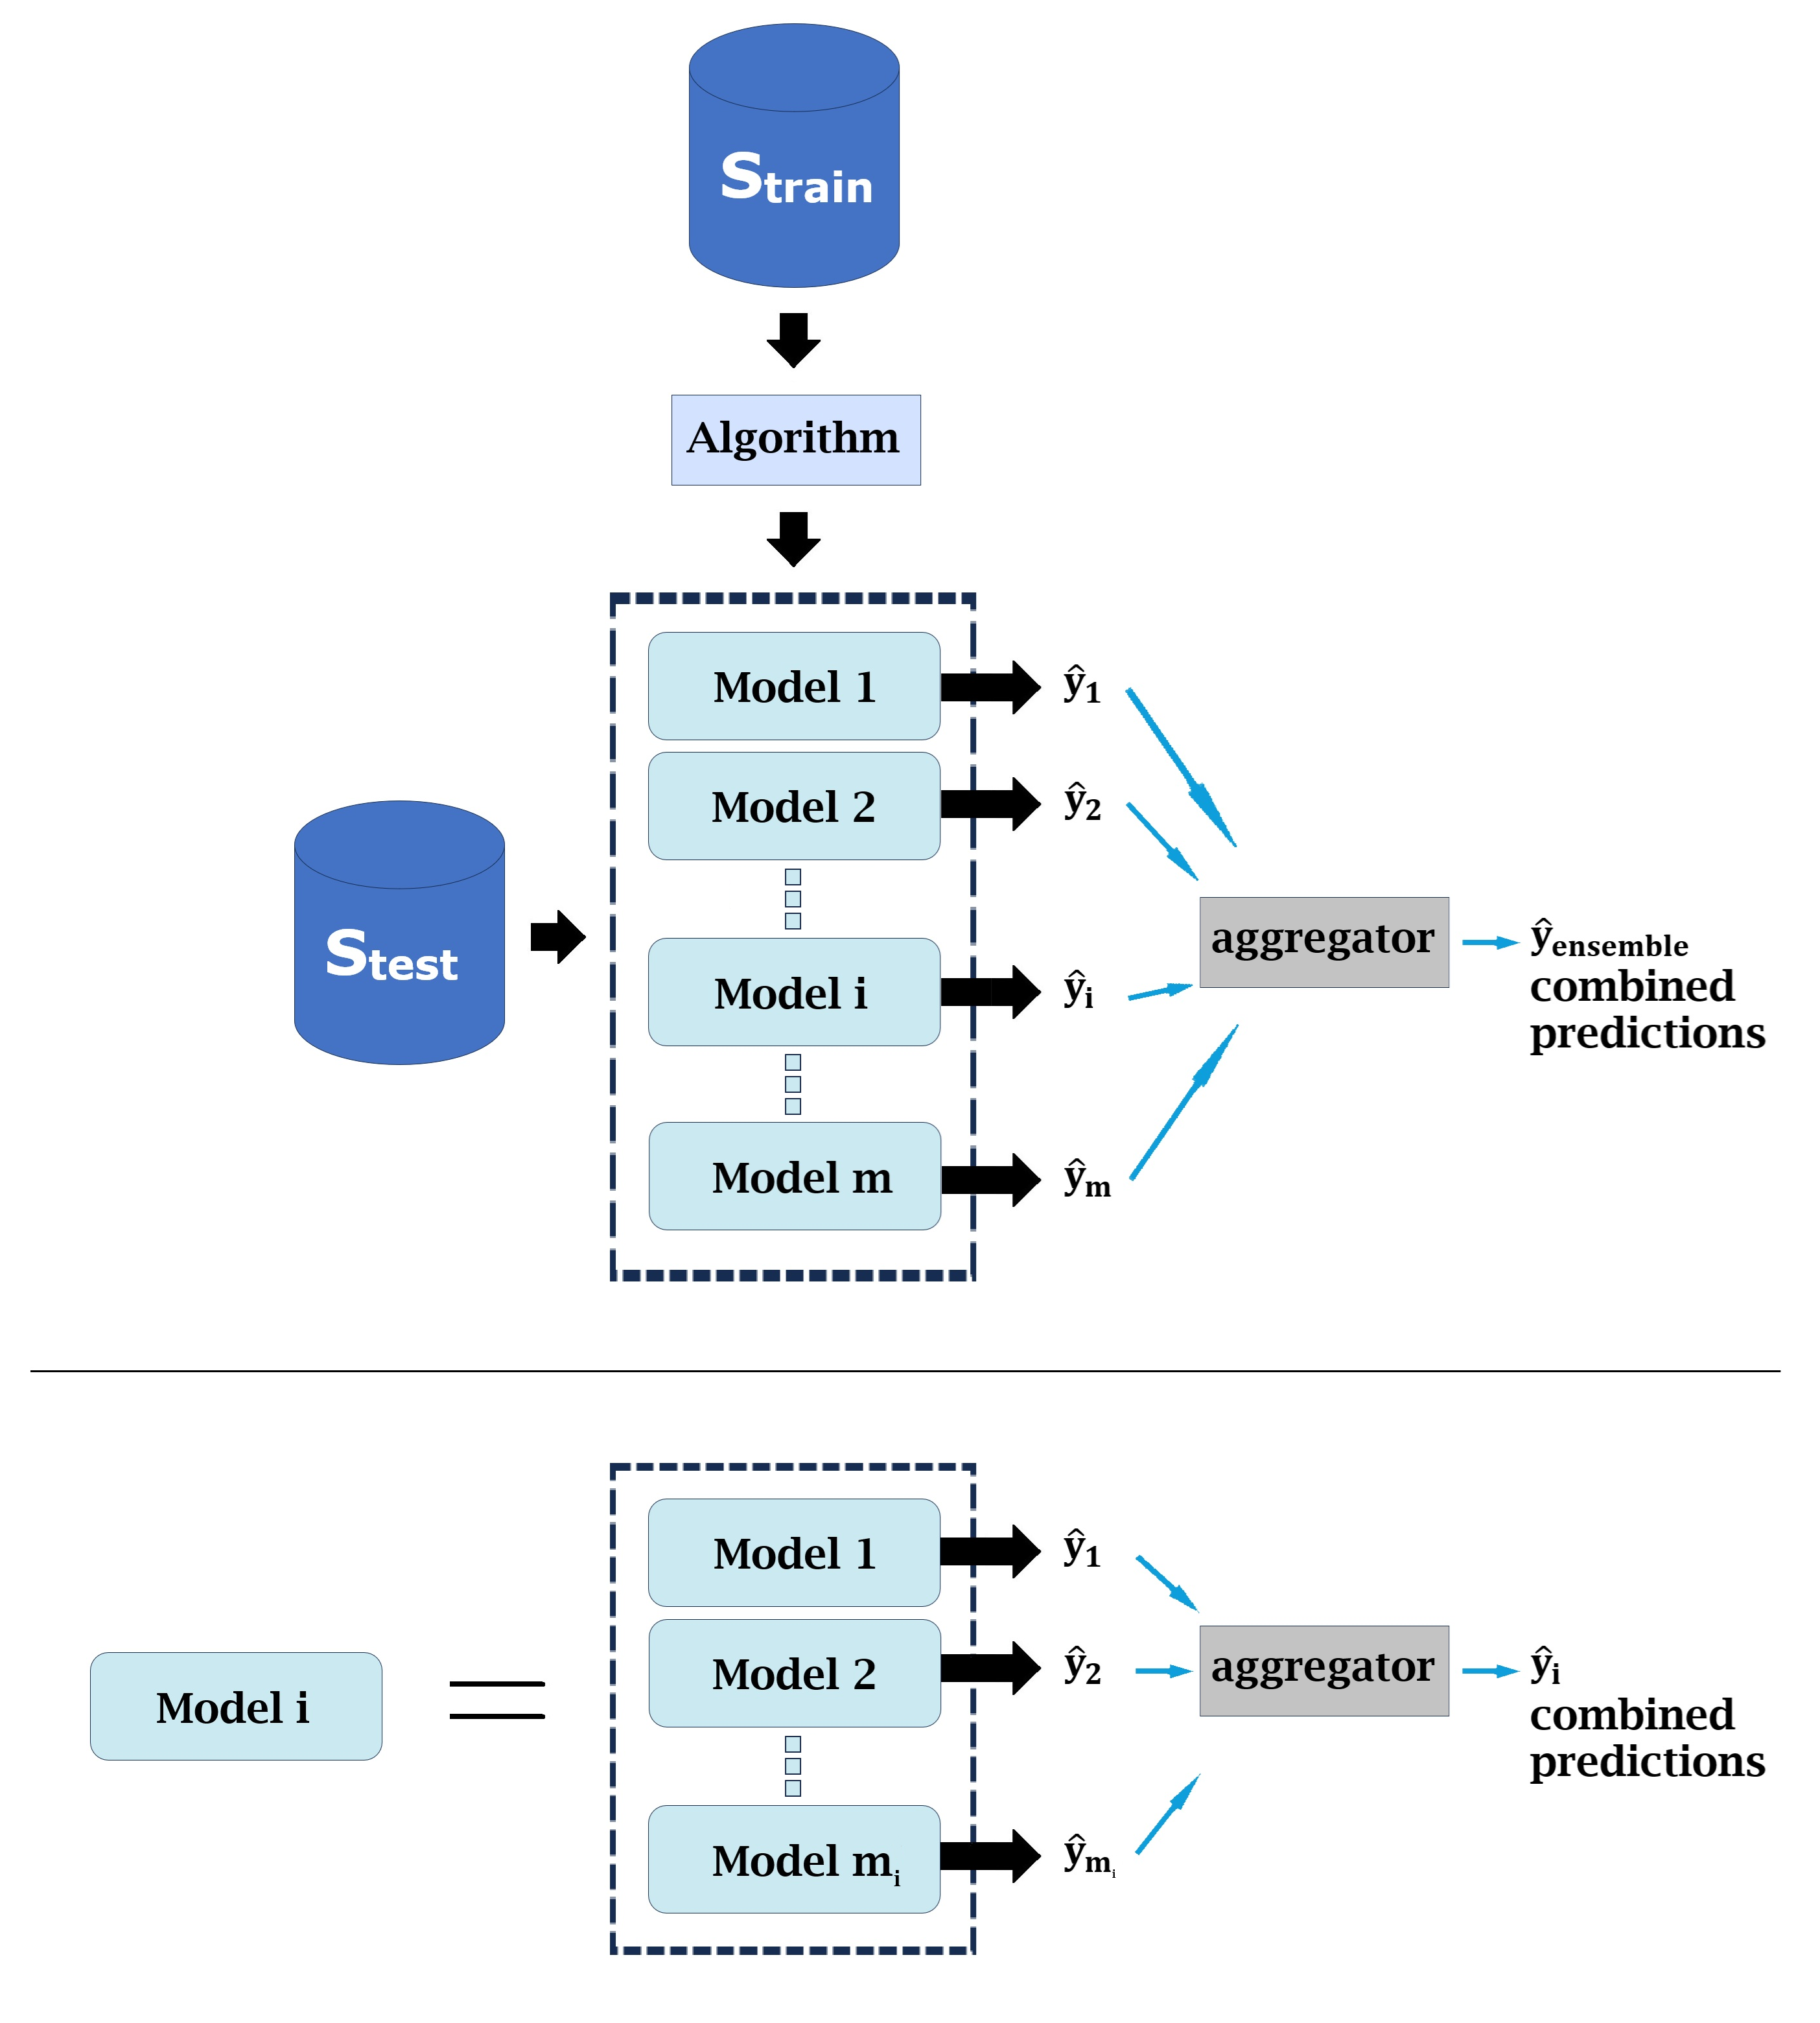
\includegraphics[width=0.64\textwidth]{img/recursive/recursive_idea.png}
    \caption{The idea of applying recursion to an ensemble model. }
    \label{fig:recursive_idea}
\end{figure}

This brings us to the next stage of our analogy: how does the quality of a decision making change if company directors no longer vote in a single room but instead, lead their own specialised sub-committees? 



\subsubsection{Representing recursively using a tree}
Each recursive architecture can be represented in the form of a tree, where each node represents an ensemble model and each edge represents a connection from this ensemble model to 1 of its base learners. Thus, there is an aggregator (can be of different types) in each node. Figure~\ref{fig:recursive_tree_example} shows an example recursive architecture. The height of the tree is $2$. It is composed of 4 ensemble models, represented by Node~2, Node~3, Node~5 and Node~6. Node~1 and Node~4 are simply particular aggregators that combine predictions from their successors. If they are neural-network-aggregators, they have different number of input features because they have different number of successors ($3$ for Node~1 and $2$ for Node~4). Node~2, Node~3, Node~5 and Node~6 consist of $m_2$, $m_3$, $m_5$ and $m_6$ base learners respectively. Each of them aggregates the predictions with their own aggregator (which can be of different types). In this experiment, $m_1 = m_2 = m_3 = m_4$ and have range $[2, 4]$. Furthermore, all nodes in the tree use the same type of aggregator but this is not a must. 

% 1 Image
\begin{figure}[H]
    \capstart
    \centering
    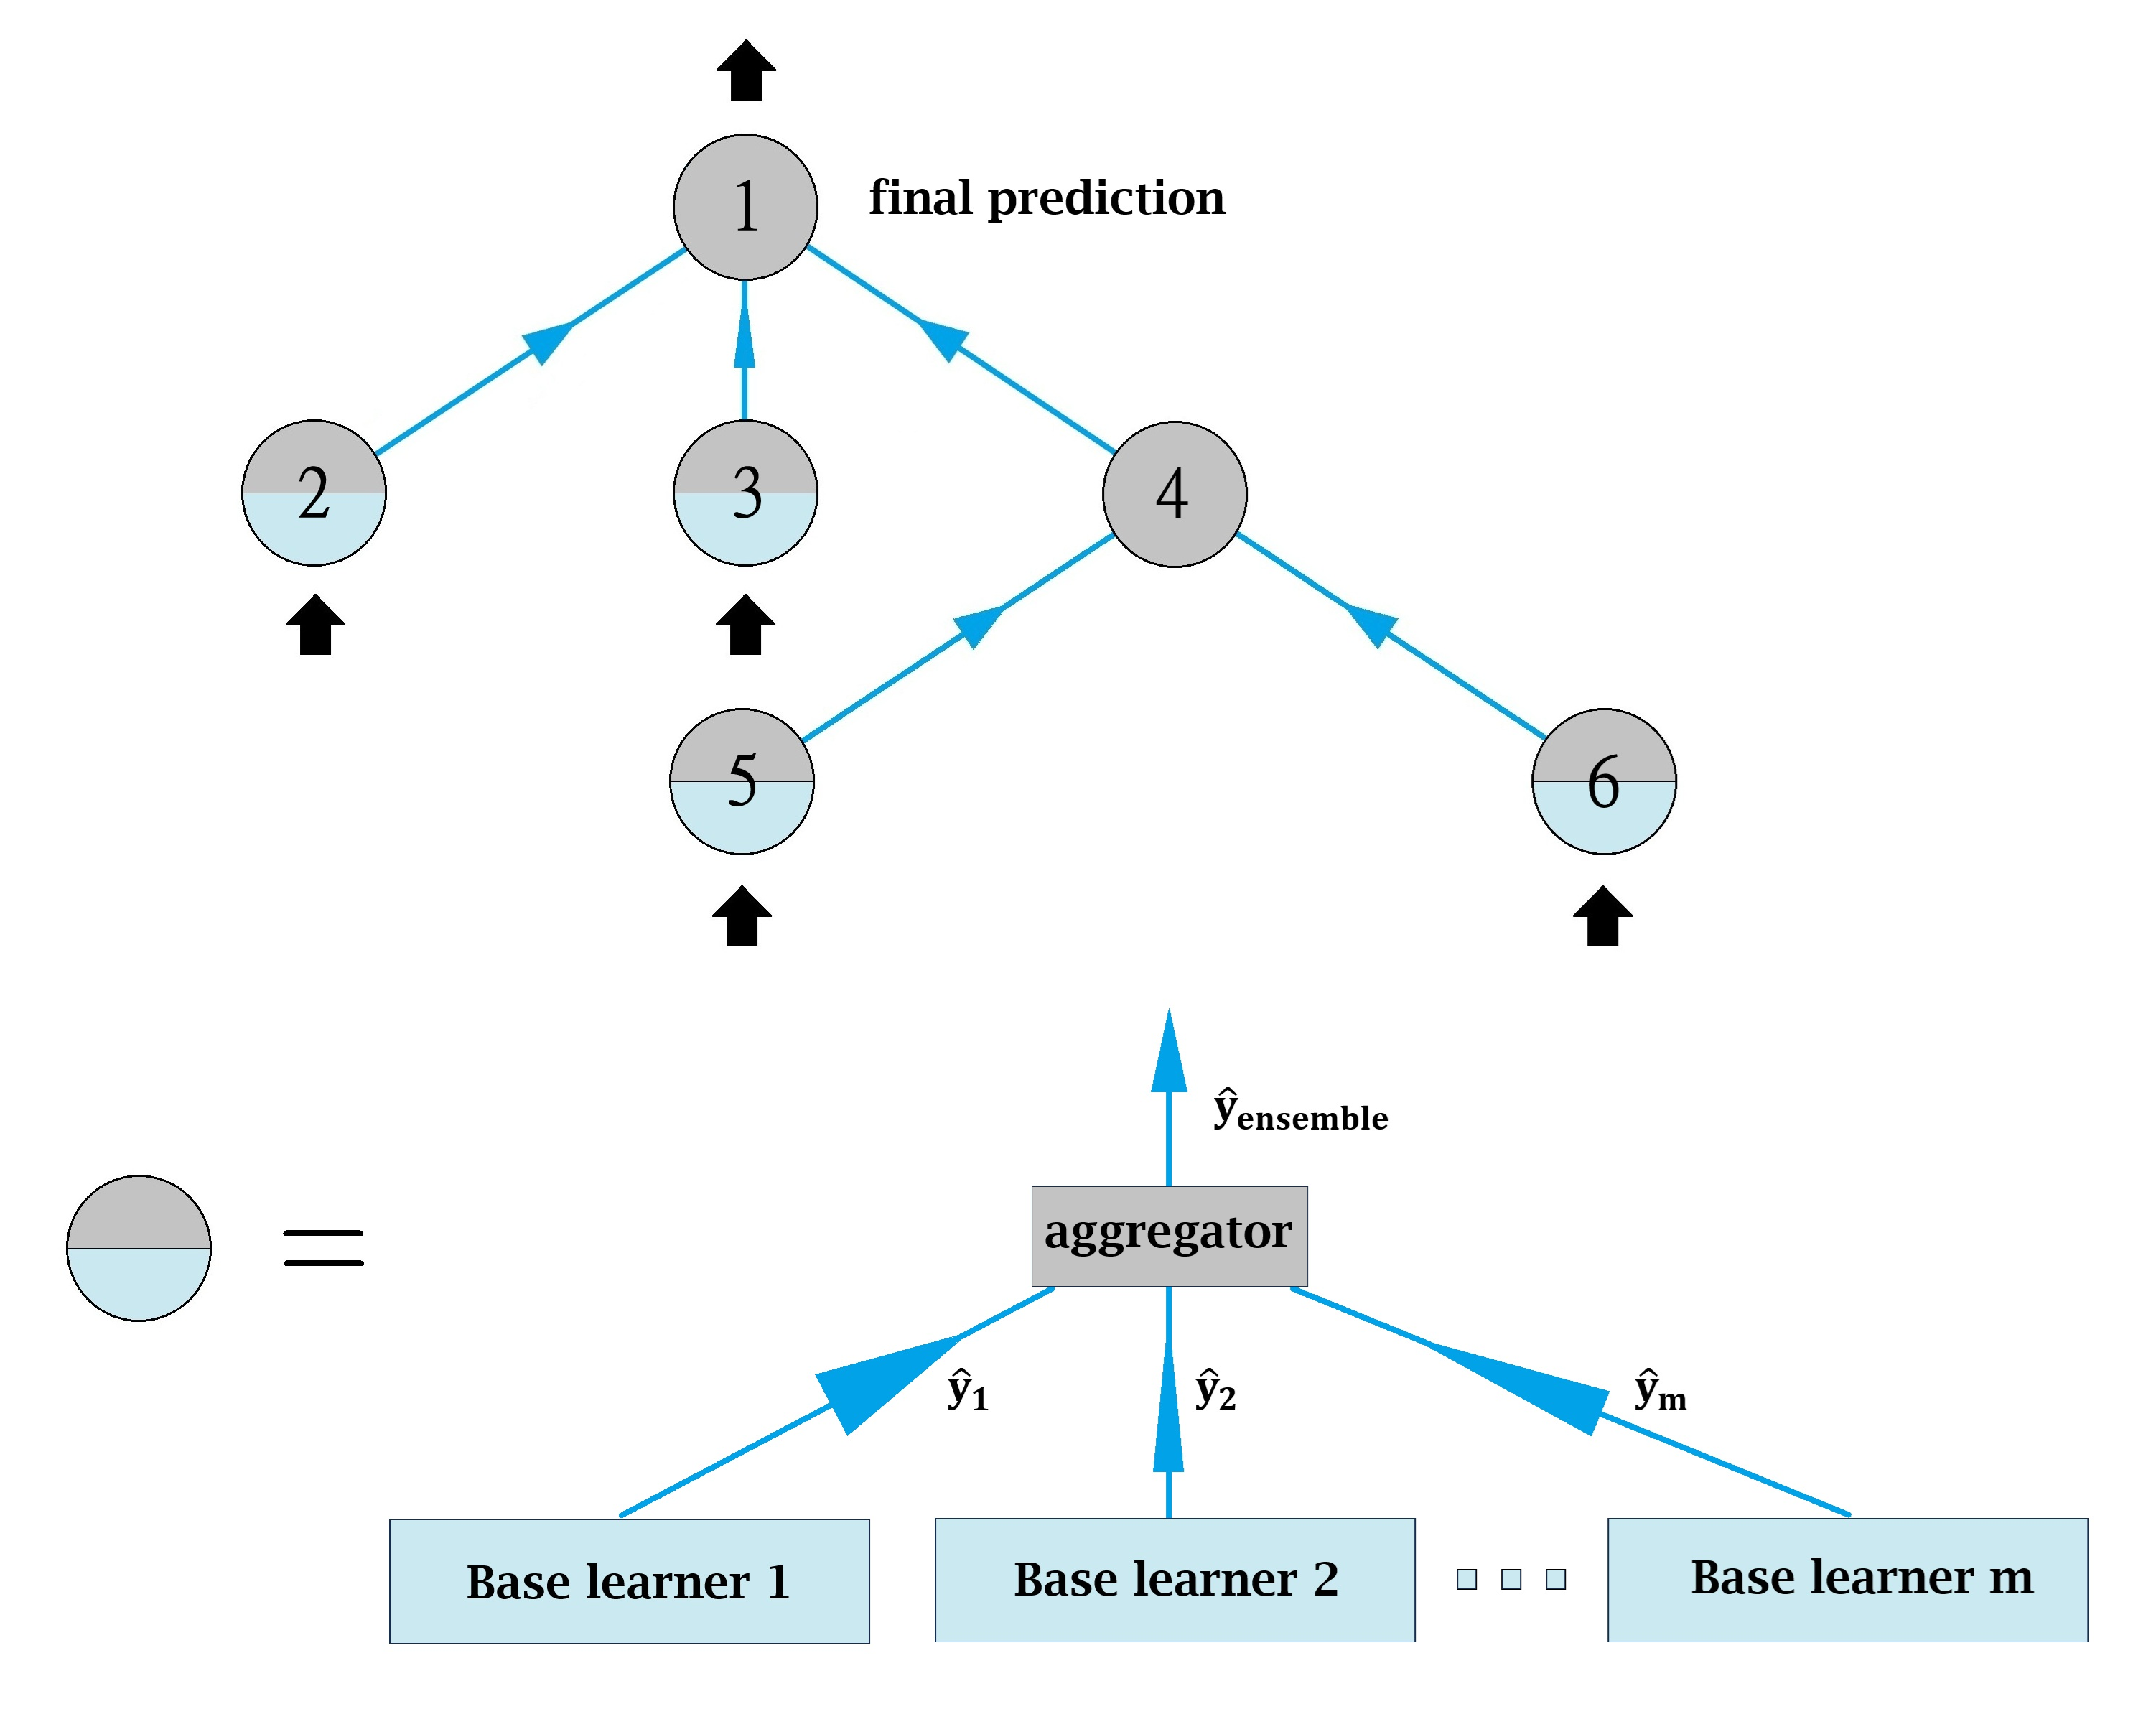
\includegraphics[width=0.64\textwidth]{img/recursive/recursive_tree_example.png}
    \caption{The tree representing an example recursive architecture of a recursive ensemble model. Each node is an instance of \texttt{RecursiveEnsembleNet}. The grey area represents an aggregator. The blue area represents an ensemble instance (e.g. \texttt{RecursiveStaticNCLEnsembleNet} instance) acting as a base learner. The blue arrows represent the data flows of predictions between \texttt{RecursiveEnsembleNet} instances. }
    \label{fig:recursive_tree_example}
\end{figure}

This is similar to the multi-layer stacker model proposed by Bosch et al.\ \cite{bosch2025multi} (Figure~2) except ``stackers'' in this project do not share the same base learners. 


\paragraph{Model Construction}
New versions of the ensemble models, \texttt{RecursiveTraditionalEnsembleNet} and 
\\
\texttt{RecursiveStaticNCLEnsembleNet}, had been created. They functioned exactly like the original versions 
\\
(\texttt{TraditionalEnsembleNet} and \texttt{StaticNCLEnsembleNet}) from Section~\ref{subsec:stage_2} and Section~\ref{subsec:stage_3} but they did not use \textit{DistributedDataParallel} or \textit{Multiprocessing}. Instead of splitting the work across two GPUs, the entire model now ran on a single GPU. 

The overall structure was managed by \texttt{RecursiveEnsembleNet}, which acted as a coordinator. It used two main components, \texttt{\_\_base\_learners} and \texttt{\_\_voter}. The \texttt{\_\_base\_learners} attribute was a list that can hold other recursive networks (non-leaf nodes) or the specific ensemble models (leaf nodes) like 
\\
\texttt{RecursiveStaticNCLEnsembleNet} or \texttt{NEATNCLEnsembleNet}. 

In this setup, each \texttt{RecursiveEnsembleNet} at a non-leaf level used its \texttt{\_\_voter} to combine the predictions coming from the layer right below it. This design allowed for a nested, hierarchical way to combine multiple different ensemble types into one final prediction. 


\paragraph{Experimental Design}
There were 2 different types of ensemble architectures used in the experiment, a \textit{perfect binary tree} and a \textit{flat tree}. Figure~\ref{fig:recursive_perfect_binary_tree} and Figure~\ref{fig:recursive_flat_tree} show their corresponding ensemble tree structures. Their ensemble performance was compared against the arithmetic-mean-ensemble in Section~\ref{subsec:stage_2} and the NCL ensemble model in Section~\ref{subsec:stage_3}. Note that $m$ of all ensemble models in this experiment were multiples of $4$ because the perfect binary tree picked was composed of 4 ensemble models. For fair comparison with a flat tree, $m$ was set to be the same, i.e. multiples of $4$. Table~\ref{table:experiment_6_varied_hyperparameters} contains all varied hyperparameters. Table~\ref{table:experiment_6_fixed_hyperparameters} contains all fixed hyperparameters. Table~\ref{table:experiment_6_metric} contains all evaluation metrics collected in this experiment. 

% 2 Image
\begin{figure}[H]
    \centering

    \begin{minipage}[t]{0.48\textwidth}
        \capstart
        \vspace{0pt}
        \centering
        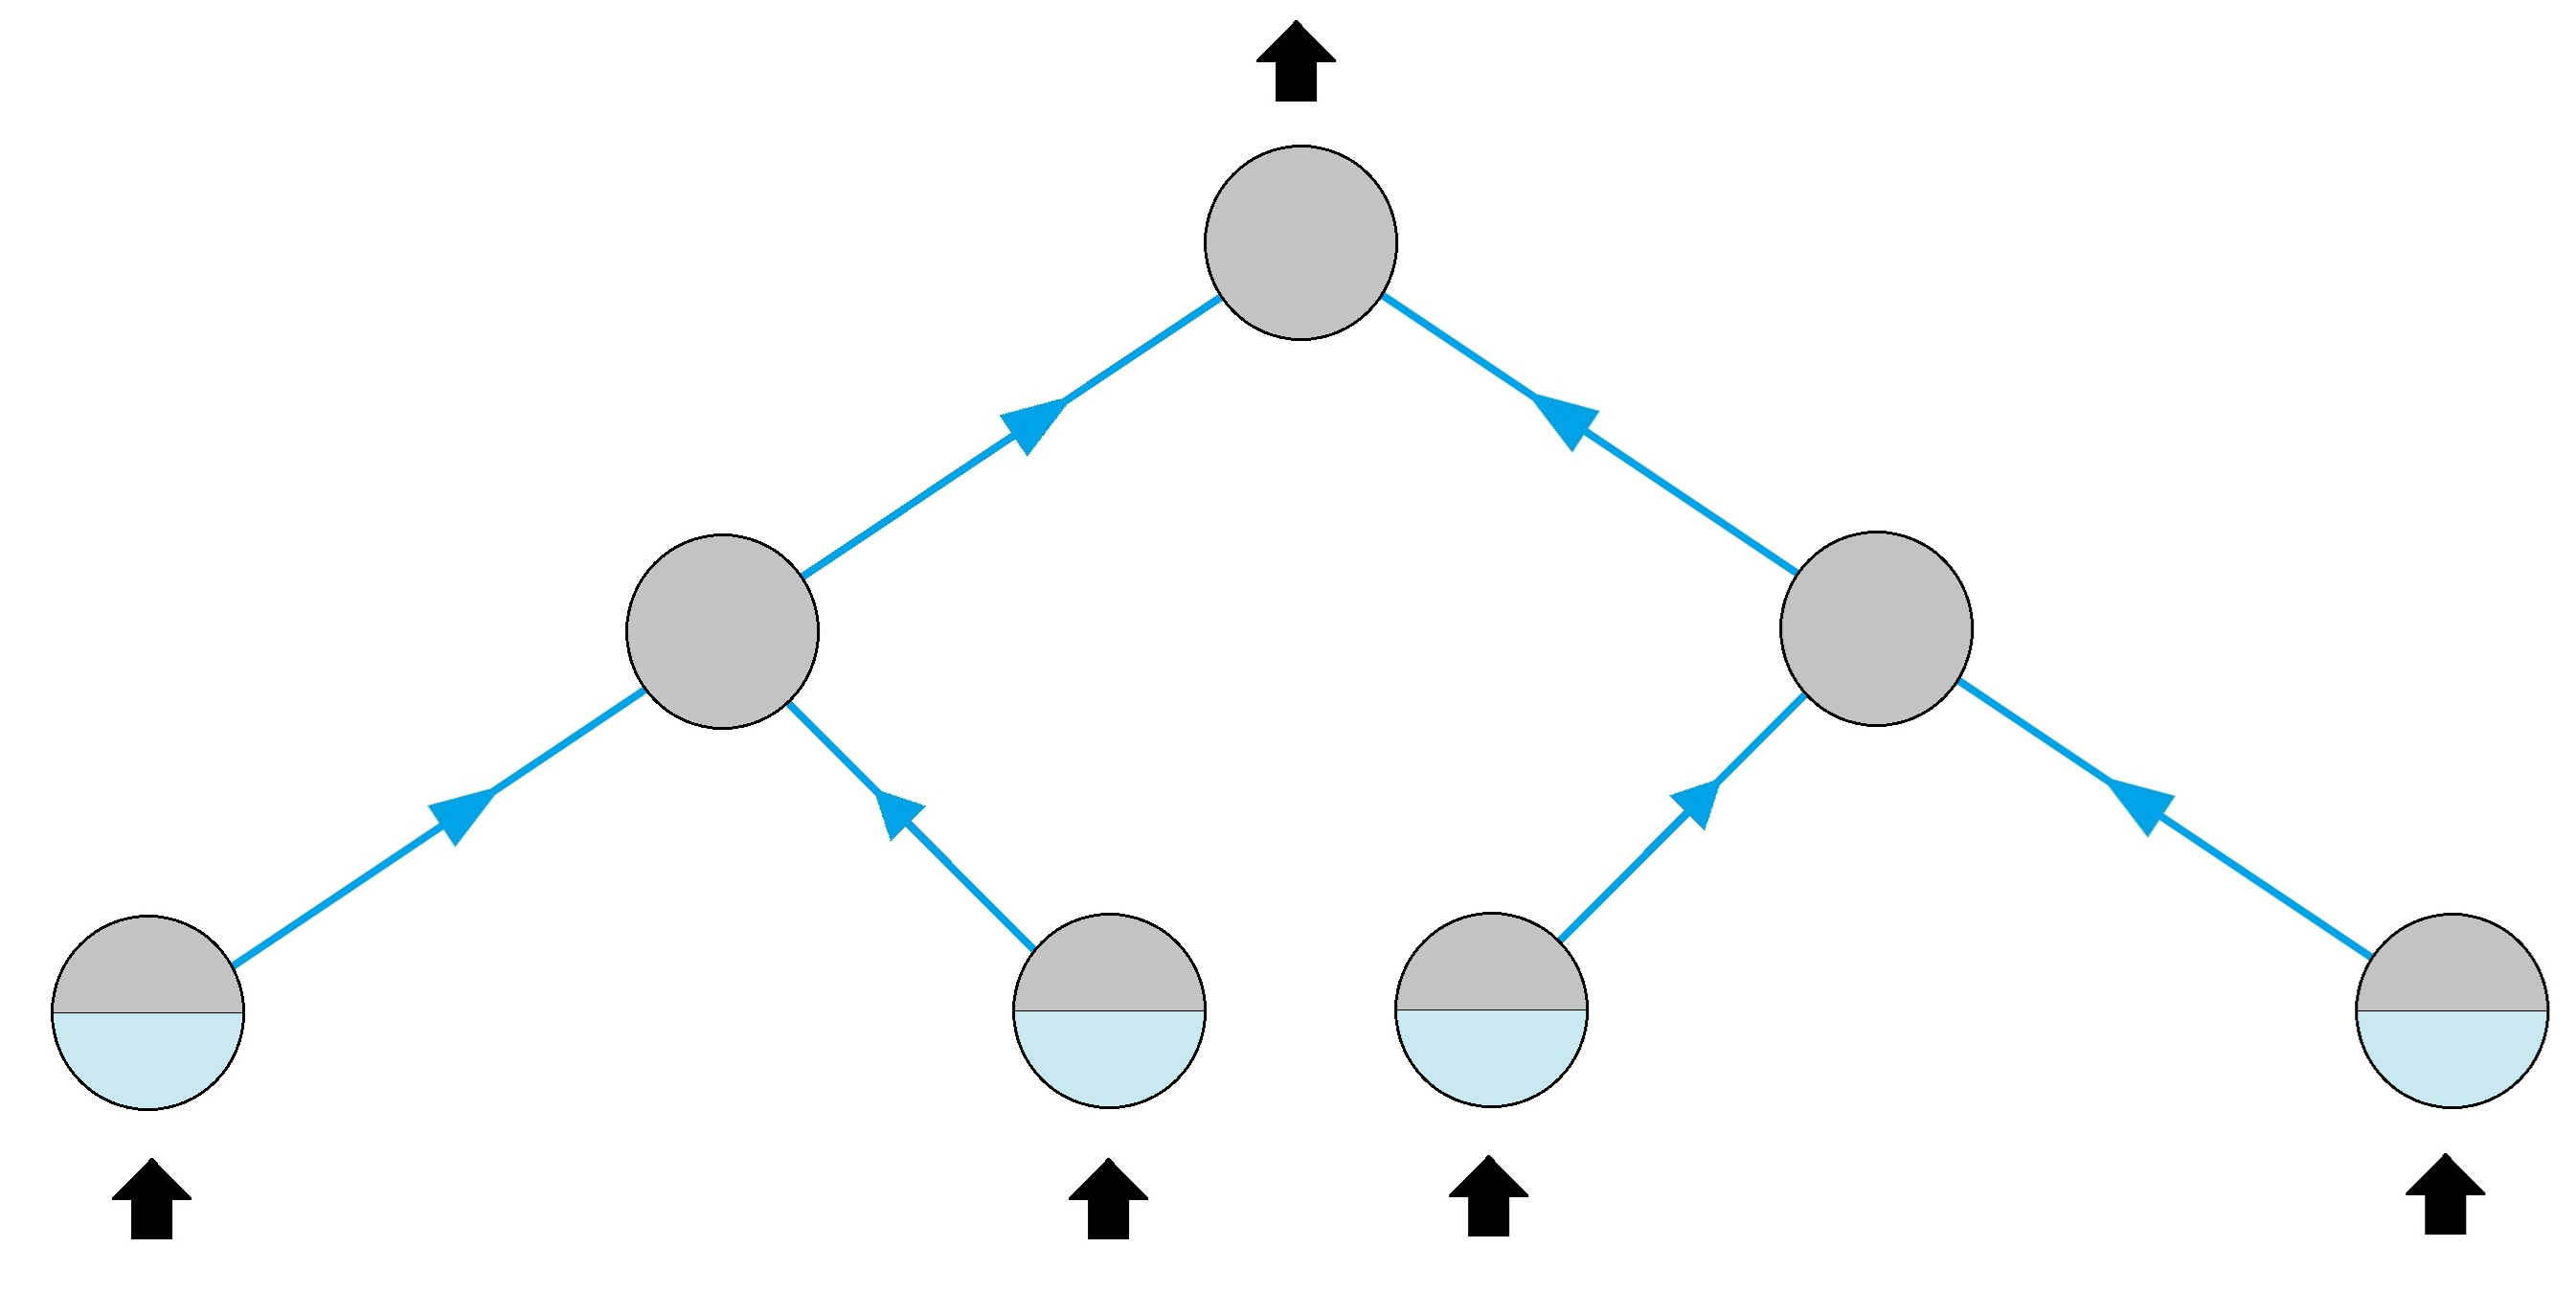
\includegraphics[width=\linewidth]{img/recursive/recursive_perfect_binary_tree.png}
        \caption{The tree representation of the recursive ensemble model whose architecture is a perfect binary tree. Each node is an instance of \texttt{RecursiveEnsembleNet}. The grey area represents an aggregator. The blue area represents an ensemble instance (e.g. \texttt{RecursiveStaticNCLEnsembleNet} instance) acting as a base learner. The blue arrows represent the data flows of predictions between \texttt{RecursiveEnsembleNet} instances. }
        \label{fig:recursive_perfect_binary_tree}
    \end{minipage}
    \hfill
    \begin{minipage}[t]{0.48\textwidth}
        \capstart
        \vspace{0pt}
        \centering
        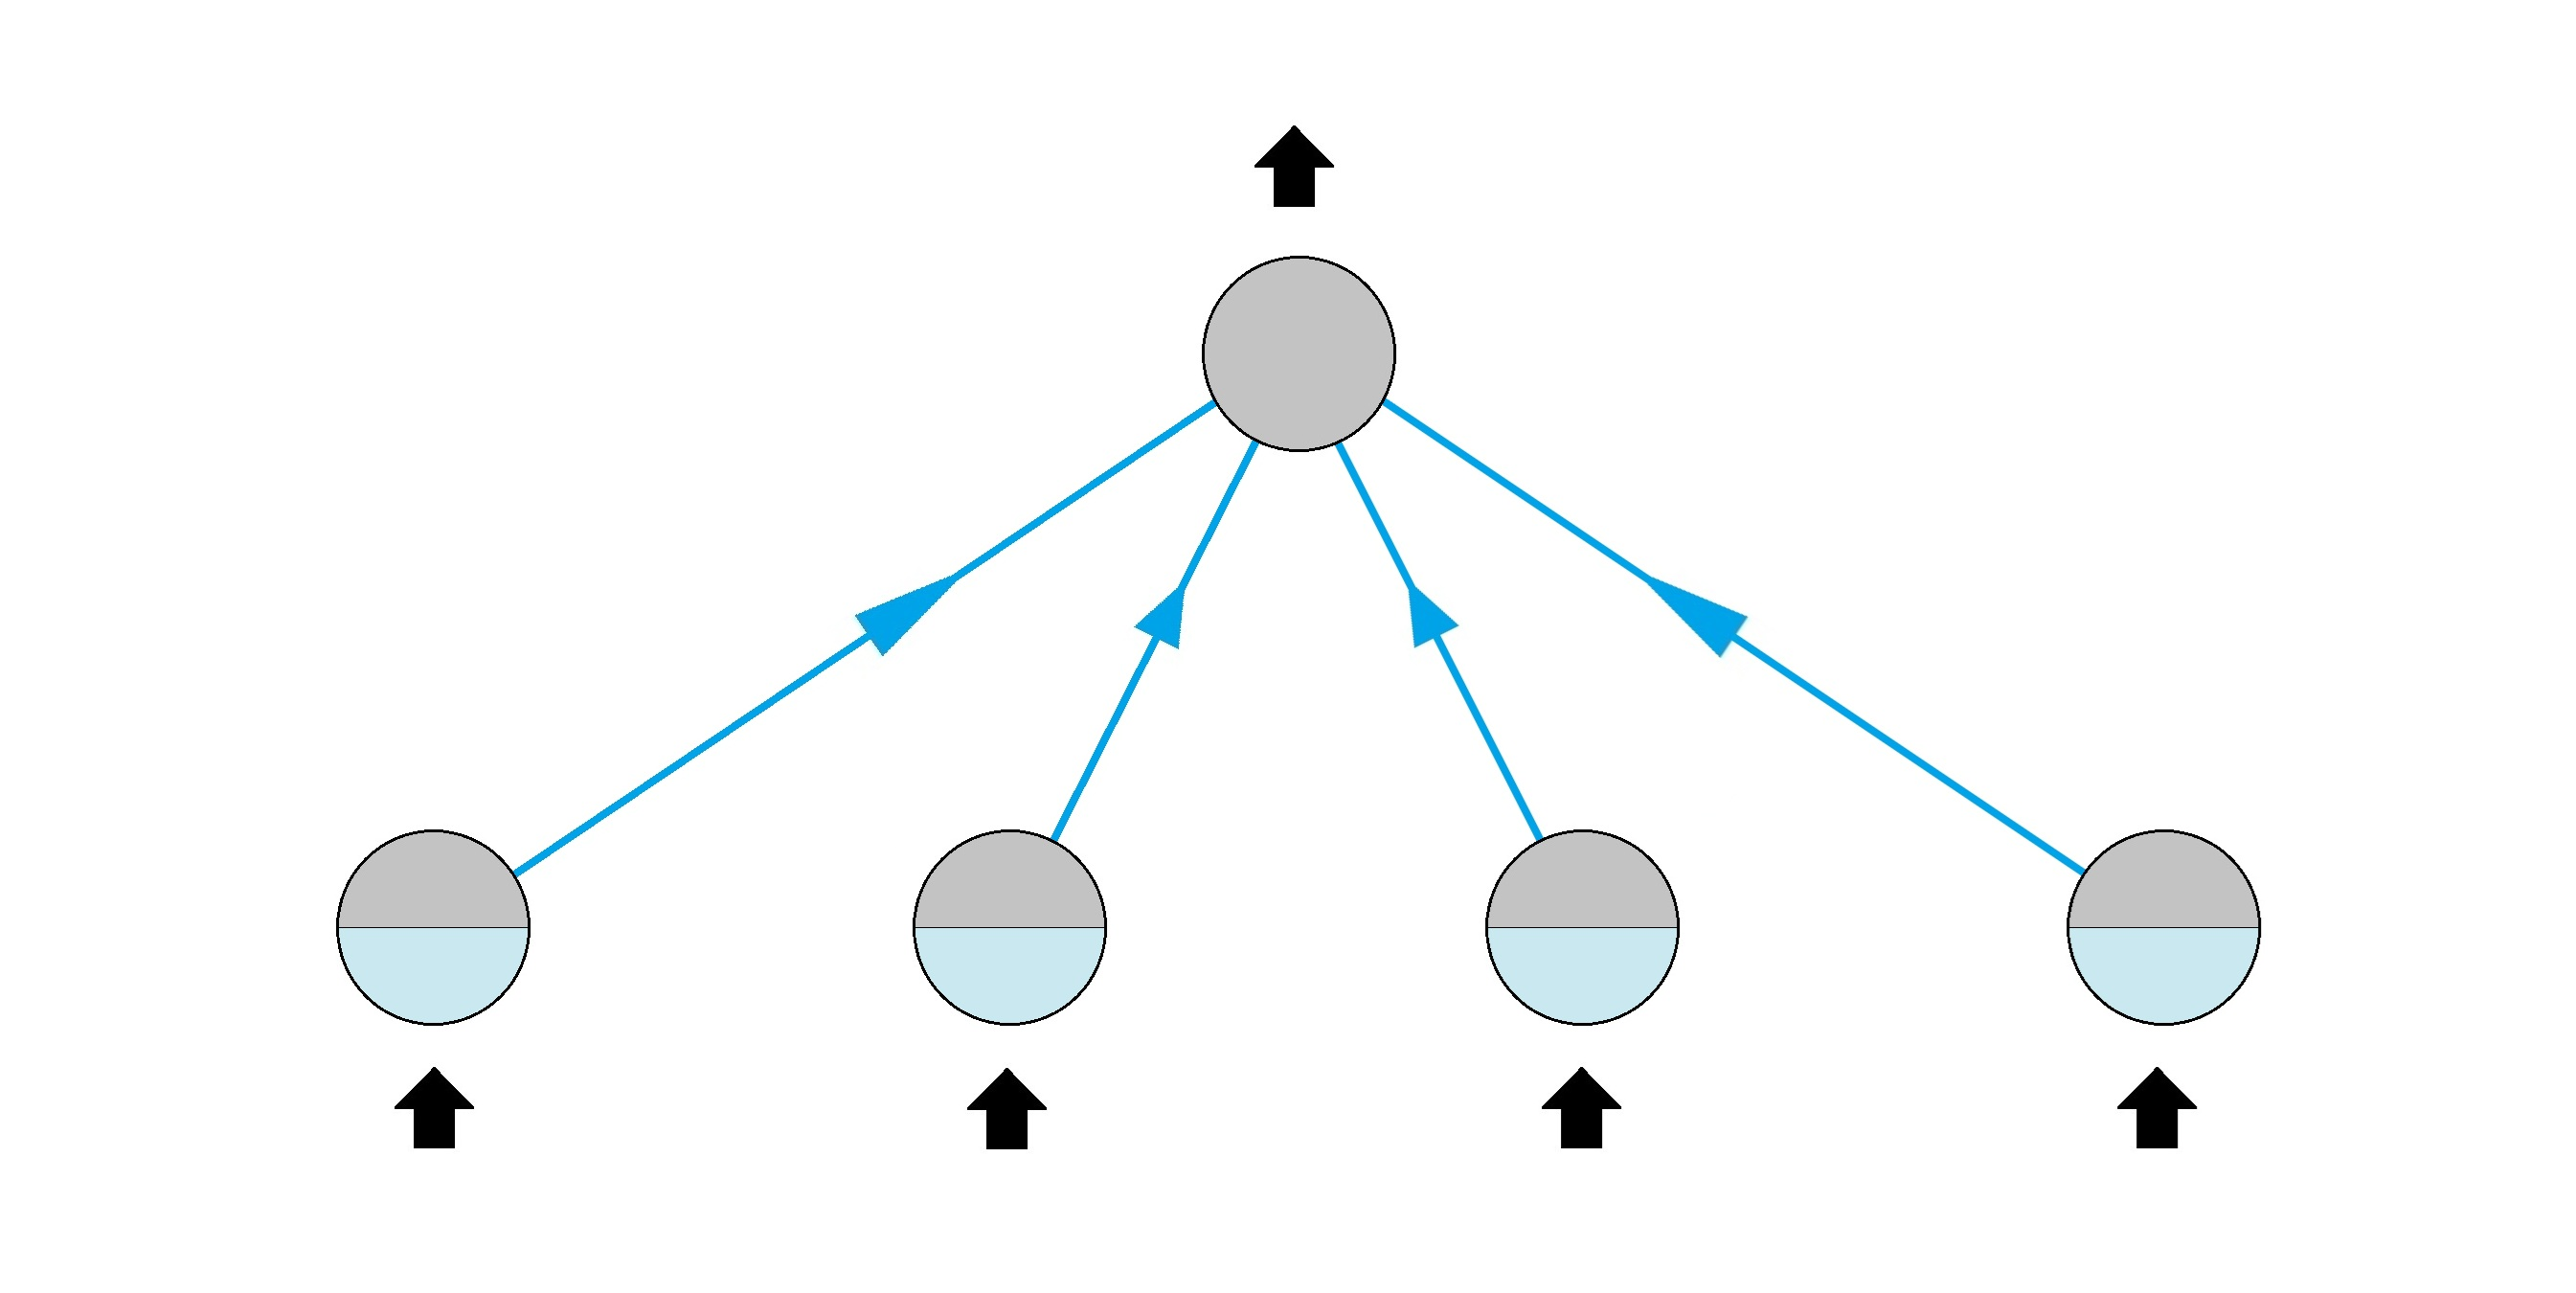
\includegraphics[width=\linewidth]{img/recursive/recursive_flat_tree.png}
        \caption{The tree representation of the recursive ensemble model whose architecture is a flat tree. Each node is an instance of \texttt{RecursiveEnsembleNet}. The grey area represents an aggregator. The blue area represents an ensemble instance (e.g. \texttt{RecursiveStaticNCLEnsembleNet} instance) acting as a base learner. The blue arrows represent the data flows of predictions between \texttt{RecursiveEnsembleNet} instances. }
        \label{fig:recursive_flat_tree}
    \end{minipage}
\end{figure}

\begin{table}[H]
    \centering
    \begin{tabular}{|c|c|p{3cm}|p{4cm}|}
        \hline
        Hyperparameter & Type & Choices / Ranges & Description \\
        \hline
        \small\texttt{architectures} & Categorical & \{perfect binary tree, flat tree\} & Ensemble model architecture \\
        \hline
        \small\texttt{correlation\_penalty\_coefficients} & Float & $[0.4, 0.9]\text{, step}=0.1$ & $\lambda$ (for NCL ensemble model only) \\
        \hline
        \small\texttt{ensemble\_sizes} & Integer & \{$[8, 16]\text{, step}=4$, $200$\} & $m$ ($200$ for recursive NEAT-NCL ensemble model and $[8, 16]$ for the others) \\
        \hline
        \small\texttt{voter} & Categorical & \{\texttt{arithmetic\_mean}, \texttt{median}, \texttt{nn}\} & Aggregator type (\texttt{nn} is not applicable to recursive NEAT-NCL ensemble model) \\
        \hline
    \end{tabular}
    \caption{Varied hyperparameters and their configurations}
    \label{table:experiment_6_varied_hyperparameters}
\end{table}

\begin{table}[H]
    \centering
    \begin{tabular}{|c|c|c|p{7cm}|}
        \hline
        Hyperparameter & Type & Choices / Ranges & Description \\
        \hline
        \small\texttt{input\_size} & Integer & $13$ & Number of input features of the MLP \\
        \hline
        \small\texttt{output\_size} & Integer & $1$ & Number of labels of the MLP \\
        \hline
        \small\texttt{optimizer} & Categorical & \texttt{torch.optim.Adam} & Optimisation algorithm used for training \\
        \hline
        \small\texttt{hidden\_sizes} & Python list & \texttt{[6]} & Model architecture (not applicable to recursive NEAT-NCL ensemble model) \\
        \hline
        \small\texttt{learning\_rate} & Float & $0.001$ & Learning rate of the optimisation algorithm \\
        \hline
        \small\texttt{dropout\_rate} & Float & $0.5$ & Dropout rate applied to the data tensor after the input layer \\
        \hline
        \small\texttt{activation} & Categorical & ReLU & Activation function used in each dense layer of the MLP \\
        \hline
        \small\texttt{epoch\_nums} & Integer & $400$ & Number of training epochs (for arithmetic-mean-ensemble and NCL ensemble model only) \\
        \hline
        \small\texttt{evolution\_epoch} & Integer & $400$ & Number of evolutionary generations during training (for recursive NEAT-NCL ensemble model only) \\
        \hline
        \small\texttt{batch\_size} & Integer & \{$32$, $506$\} & Number of training samples passed to the model in one go ($506$ for recursive NEAT-NCL ensemble model and $32$ for the others) \\
        \hline
    \end{tabular}
    \caption{Fixed hyperparameters and their configurations}
    \label{table:experiment_6_fixed_hyperparameters}
\end{table}

\begin{table}[H]
    \centering
    \begin{tabular}{|c|c|c|}
        \hline
        Metric & Type & Description \\
        \hline
        \small\texttt{loss\_test} & Float & MSE of ensemble model during testing \\
        \hline
    \end{tabular}
    \caption{Evaluation metrics}
    \label{table:experiment_6_metric}
\end{table}